
\documentclass{beamer}
\usetheme{ucl}

%%% Increase the height of the banner: the argument is a scale factor >=1.0
%\setbeamertemplate{banner}[ucl][0.1]

%%% Change the colour of the main banner
%%% The background should be one of the UCL colours (except pink or white):
%%%   black,darkpurple,darkred,darkblue,darkgreen,darkbrown,richred,midred,
%%%   navyblue,midgreen,darkgrey,orange,brightblue,brightgreen,lightgrey,
%%%   lightpurple,yellow,lightblue,lightgreen,stone
\setbeamercolor{banner}{bg=darkpurple}
%\setbeamercolor{banner}{bg=yellow,fg=black}

%%% Add a stripe behind the banner
%\setbeamercolor{banner stripe}{bg=darkpurple,fg=black}

%%% The main structural elements
\setbeamercolor{structure}{fg=black}

%%% Author/Title/Date and slide number in the footline
\setbeamertemplate{footline}[author title date]

%%% Puts the section/subsection in the headline
% \setbeamertemplate{headline}[section]

%%% Puts a navigation bar on top of the banner
%%% For this to work correctly, the each \section command needs to be
%%% followed by a \subsection. Requires one extra compile.
% \setbeamertemplate{headline}[miniframes]
%%% Accepts an optional argument determining the width
% \setbeamertemplate{headline}[miniframes][0.3\paperwidth]


%%% Puts the frame title in the banner
%%% Won't work correctly with the above headline templates
%\useoutertheme{ucltitlebanner}
%%% Similar to above, but smaller (and puts subtitle on same line as title)
\useoutertheme[small]{ucltitlebanner}

%%% Gives block elements (theorems, examples) a border
% \useinnertheme{blockborder}
%%% Sets the body of block elements to be clear
% \setbeamercolor{block body}{bg=white,fg=black}

%%% Include CSML logo on title slide
%\titlegraphic{\includegraphics[width=0.16\paperwidth]{csml_logo}}

%%% Include CSML logo in bottom right corner of all slides
%\logo{\includegraphics[width=0.12\paperwidth]{csml_logo}}

%%% Set a background colour
% \setbeamercolor{background canvas}{bg=lightgrey}

%%% Set a background image
%%% Some sample images are available from the UCL image store:
%%%   https://www.imagestore.ucl.ac.uk/home/start
% \setbeamertemplate{background canvas}{%
%   \includegraphics[width=\paperwidth]{imagename}}



%%%%%% Some other settings that can make things look nicer
%%% Set a smaller indent for description environment
\setbeamersize{description width=2em}
%%% Remove nav symbols (and shift any logo down to corner)
\setbeamertemplate{navigation symbols}{\vspace{-2ex}}








\DeclareMathOperator{\Cov}{Cov}
\DeclareMathOperator{\Var}{Var}
\DeclareMathOperator{\E}{\mathbb{E}}
\DeclareMathOperator{\Proba}{\mathbb{P}}

\newcommand{\Covb}[2]{\ensuremath{\Cov\!\left[#1,#2\right]}}
\newcommand{\Eb}[1]{\ensuremath{\E\!\left[#1\right]}}
\newcommand{\Pb}[1]{\ensuremath{\Proba\!\left[#1\right]}}
\newcommand{\Varb}[1]{\ensuremath{\Var\!\left[#1\right]}}

% norm
\newcommand{\norm}[1]{\| #1 \|}

\newcommand{\indep}{\rotatebox[origin=c]{90}{$\models$}}





\usepackage{mathptmx,amsmath,amssymb,graphicx,bibentry,bbm,ragged2e}
\usepackage[english]{babel}

\makeatletter

\newcommand{\noun}[1]{\textsc{#1}}
\newcommand{\jitem}[1]{\item \begin{justify} #1 \end{justify} \vfill{}}
\newcommand{\sframe}[2]{\frame{\frametitle{#1} #2}}

\newenvironment{centercolumns}{\begin{columns}[c]}{\end{columns}}
%\newenvironment{jitem}{\begin{justify}\begin{itemize}}{\end{itemize}\end{justify}}



%\usetheme{Warsaw}
%\setbeamertemplate{footline}[text line]{}
%\setbeamertemplate{headline}{}
%\setbeamercolor{structure}{fg=purple!50!blue, bg=purple!50!blue}

%\setbeamersize{text margin left=15pt,text margin right=15pt}

%\setbeamercovered{transparent}


\@ifundefined{showcaptionsetup}{}{%
 \PassOptionsToPackage{caption=false}{subfig}}
\usepackage{subfig}

\usepackage[utf8]{inputenc}
\usepackage[T1]{fontenc}

\usepackage{multirow}


\makeatother

\def \draft {1}

\usepackage{xparse}
\usepackage{ifthen}
\DeclareDocumentCommand{\comment}{m o o o o}
{\ifthenelse{\draft=1}{
    \textcolor{red}{\textbf{C : }#1}
    \IfValueT{#2}{\textcolor{blue}{\textbf{A1 : }#2}}
    \IfValueT{#3}{\textcolor{ForestGreen}{\textbf{A2 : }#3}}
    \IfValueT{#4}{\textcolor{red!50!blue}{\textbf{A3 : }#4}}
    \IfValueT{#5}{\textcolor{Aquamarine}{\textbf{A4 : }#5}}
 }{}
}
\newcommand{\todo}[1]{
\ifthenelse{\draft=1}{\textcolor{red!50!blue}{\textbf{TODO : \textit{#1}}}}{}
}




\begin{document}

\title[Urban evolution and co-evolution]{Modeling urban evolution and co-evolution in systems of cities}
\author[Raimbault]{J.~Raimbault$^{1,2,3\ast}$\\\medskip
$^{\ast}$\texttt{j.raimbault@ucl.ac.uk}
}

\institute[UCL]{$^{1}$Center for Advanced Spatial Analysis, University College London\\
$^{2}$UPS CNRS 3611 Complex Systems Institute Paris\\
$^{3}$UMR CNRS 8504 G{\'e}ographie-cit{\'e}s
}


\date[July 18th 2020]{Urban Genome Project seminar\\
University of Toronto, School of Cities\\
December 9th 2020
}

\frame{\maketitle}

\AtBeginSection[]
{
	\frame{
		\tableofcontents[currentsection, hideallsubsections]
	}
	\addtocounter{framenumber}{-1}
}


%\sframe{Contents}{
%
%	\tableofcontents
%
%}







\section{Urban evolutionary theory}

% Systems of cities are adaptive complex systems, which have been theorised and modelled from many viewpoints and by different disciplines. Understanding the processes driving their dynamics is a crucial challenge for sustainable urban and territorial planning. The concept of urban evolution has proved relevant in this regard. This presentation summarises recent results obtained within the frame of the Evolutionary Urban Theory, a geographical approach to urban systems dynamics developed for more than 20 years by Denise Pumain and collaborators. We first review the main theoretical assumptions underlying this theory and results obtained with different simulation models in previous works. We also highlight the role of new model exploration and validation practices and tools developed in that context, implemented in the OpenMOLE platform.



\sframe{Urban evolution: Urban systems and Artificial Life}{


\begin{center}
	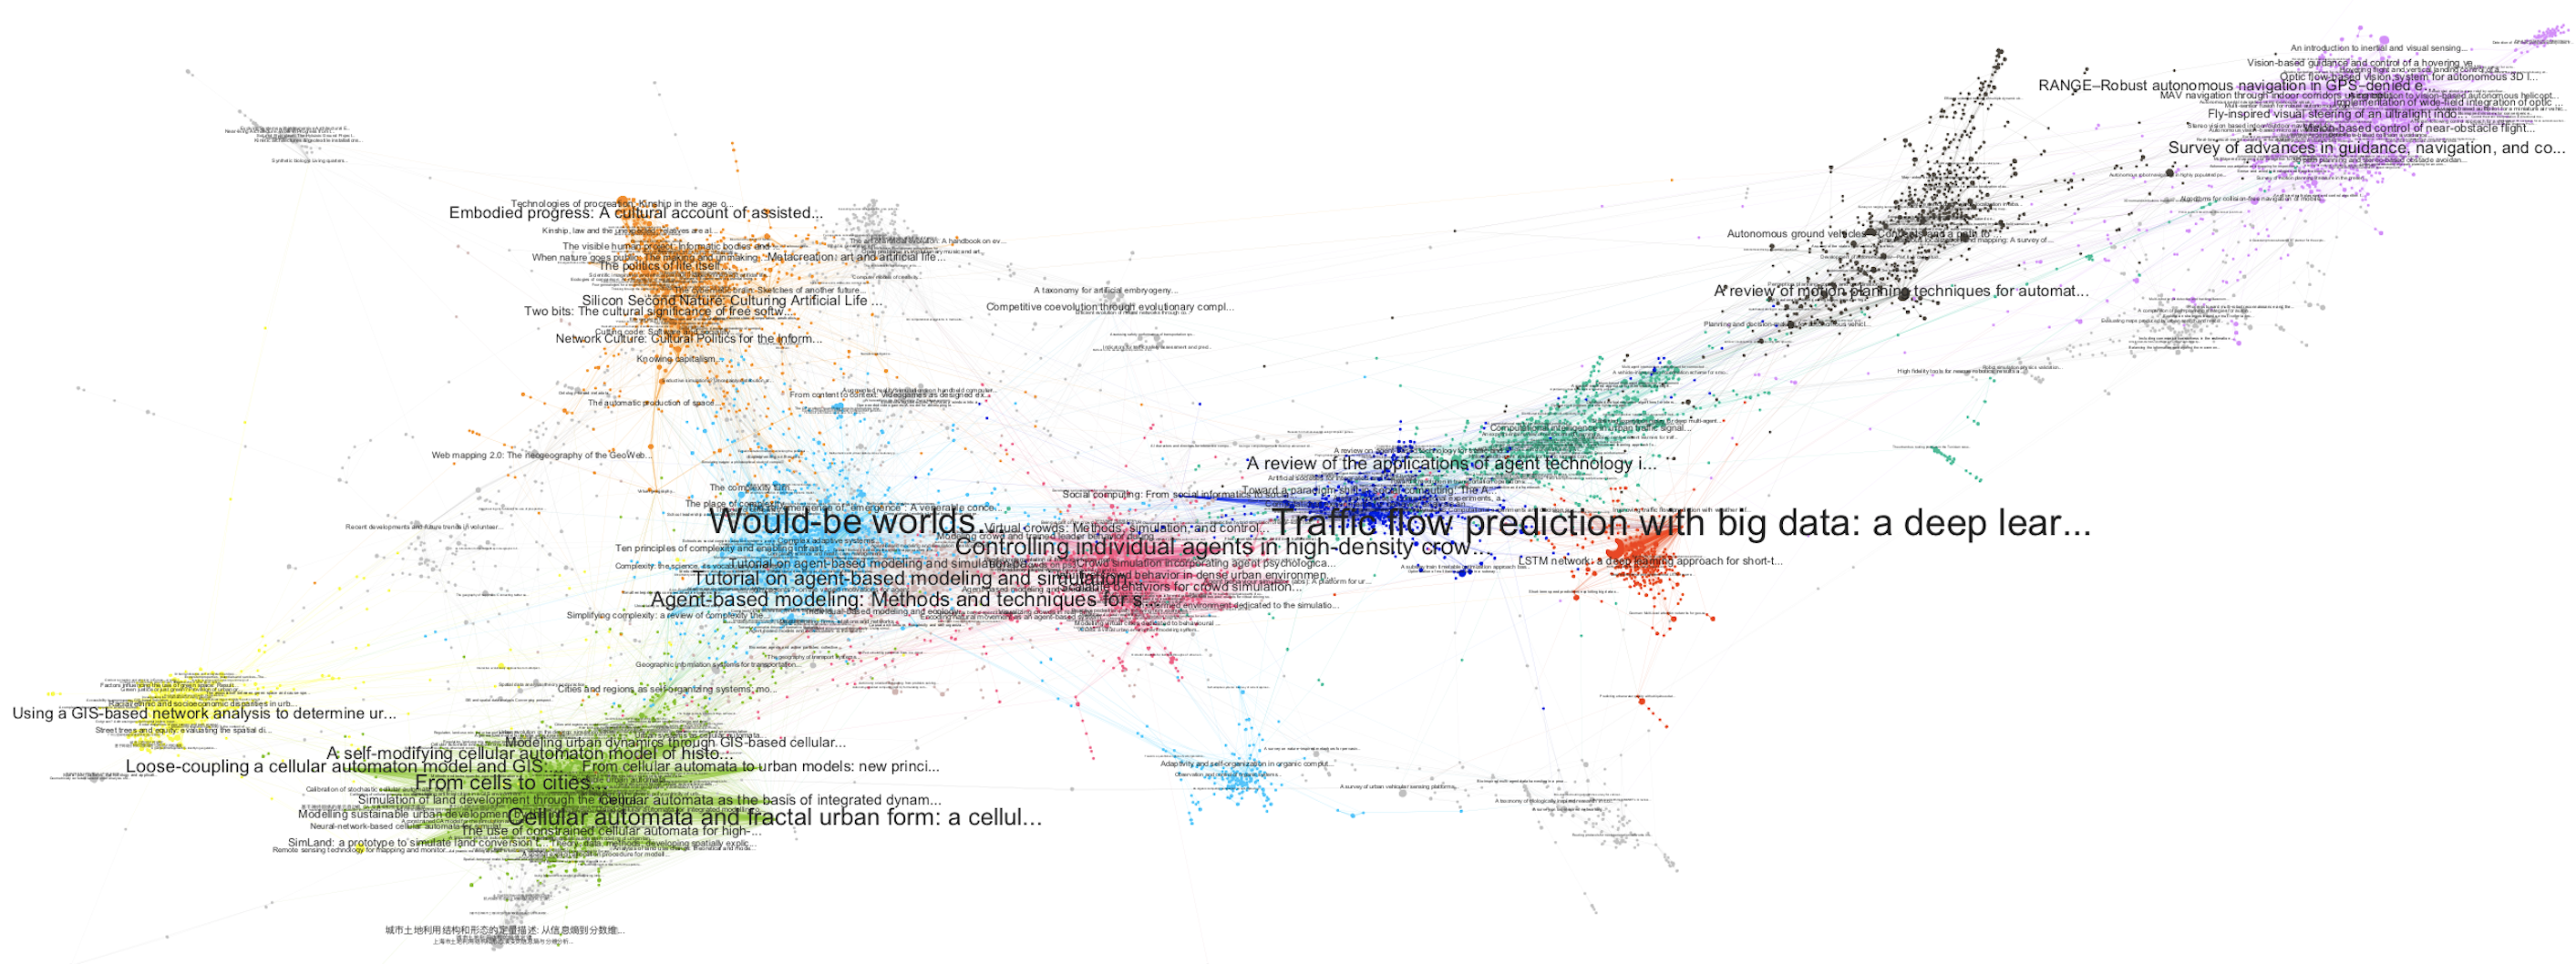
\includegraphics[width=\linewidth]{../../../Communications/ALife2020/figures/corealife_zoom.png}
\end{center}

{\footnotesize \textit{Citation network of ALife studies of urban systems} \cite{raimbault2020cities} arXiv:2002.12926}

\medskip

\textbf{Transfer of concepts: } Urban morphogenesis, bio-inspired design, urban ecology, autopoiesis \cite{batty2009centenary}

}


\sframe{Urban Evolution}{

\justify

\textbf{Urban evolution} extending cultural evolution, cities as agents with their proper genome and evolutionary dynamics?

\medskip

\begin{center}
	\begin{columns}
	\begin{column}{0.45\linewidth}
	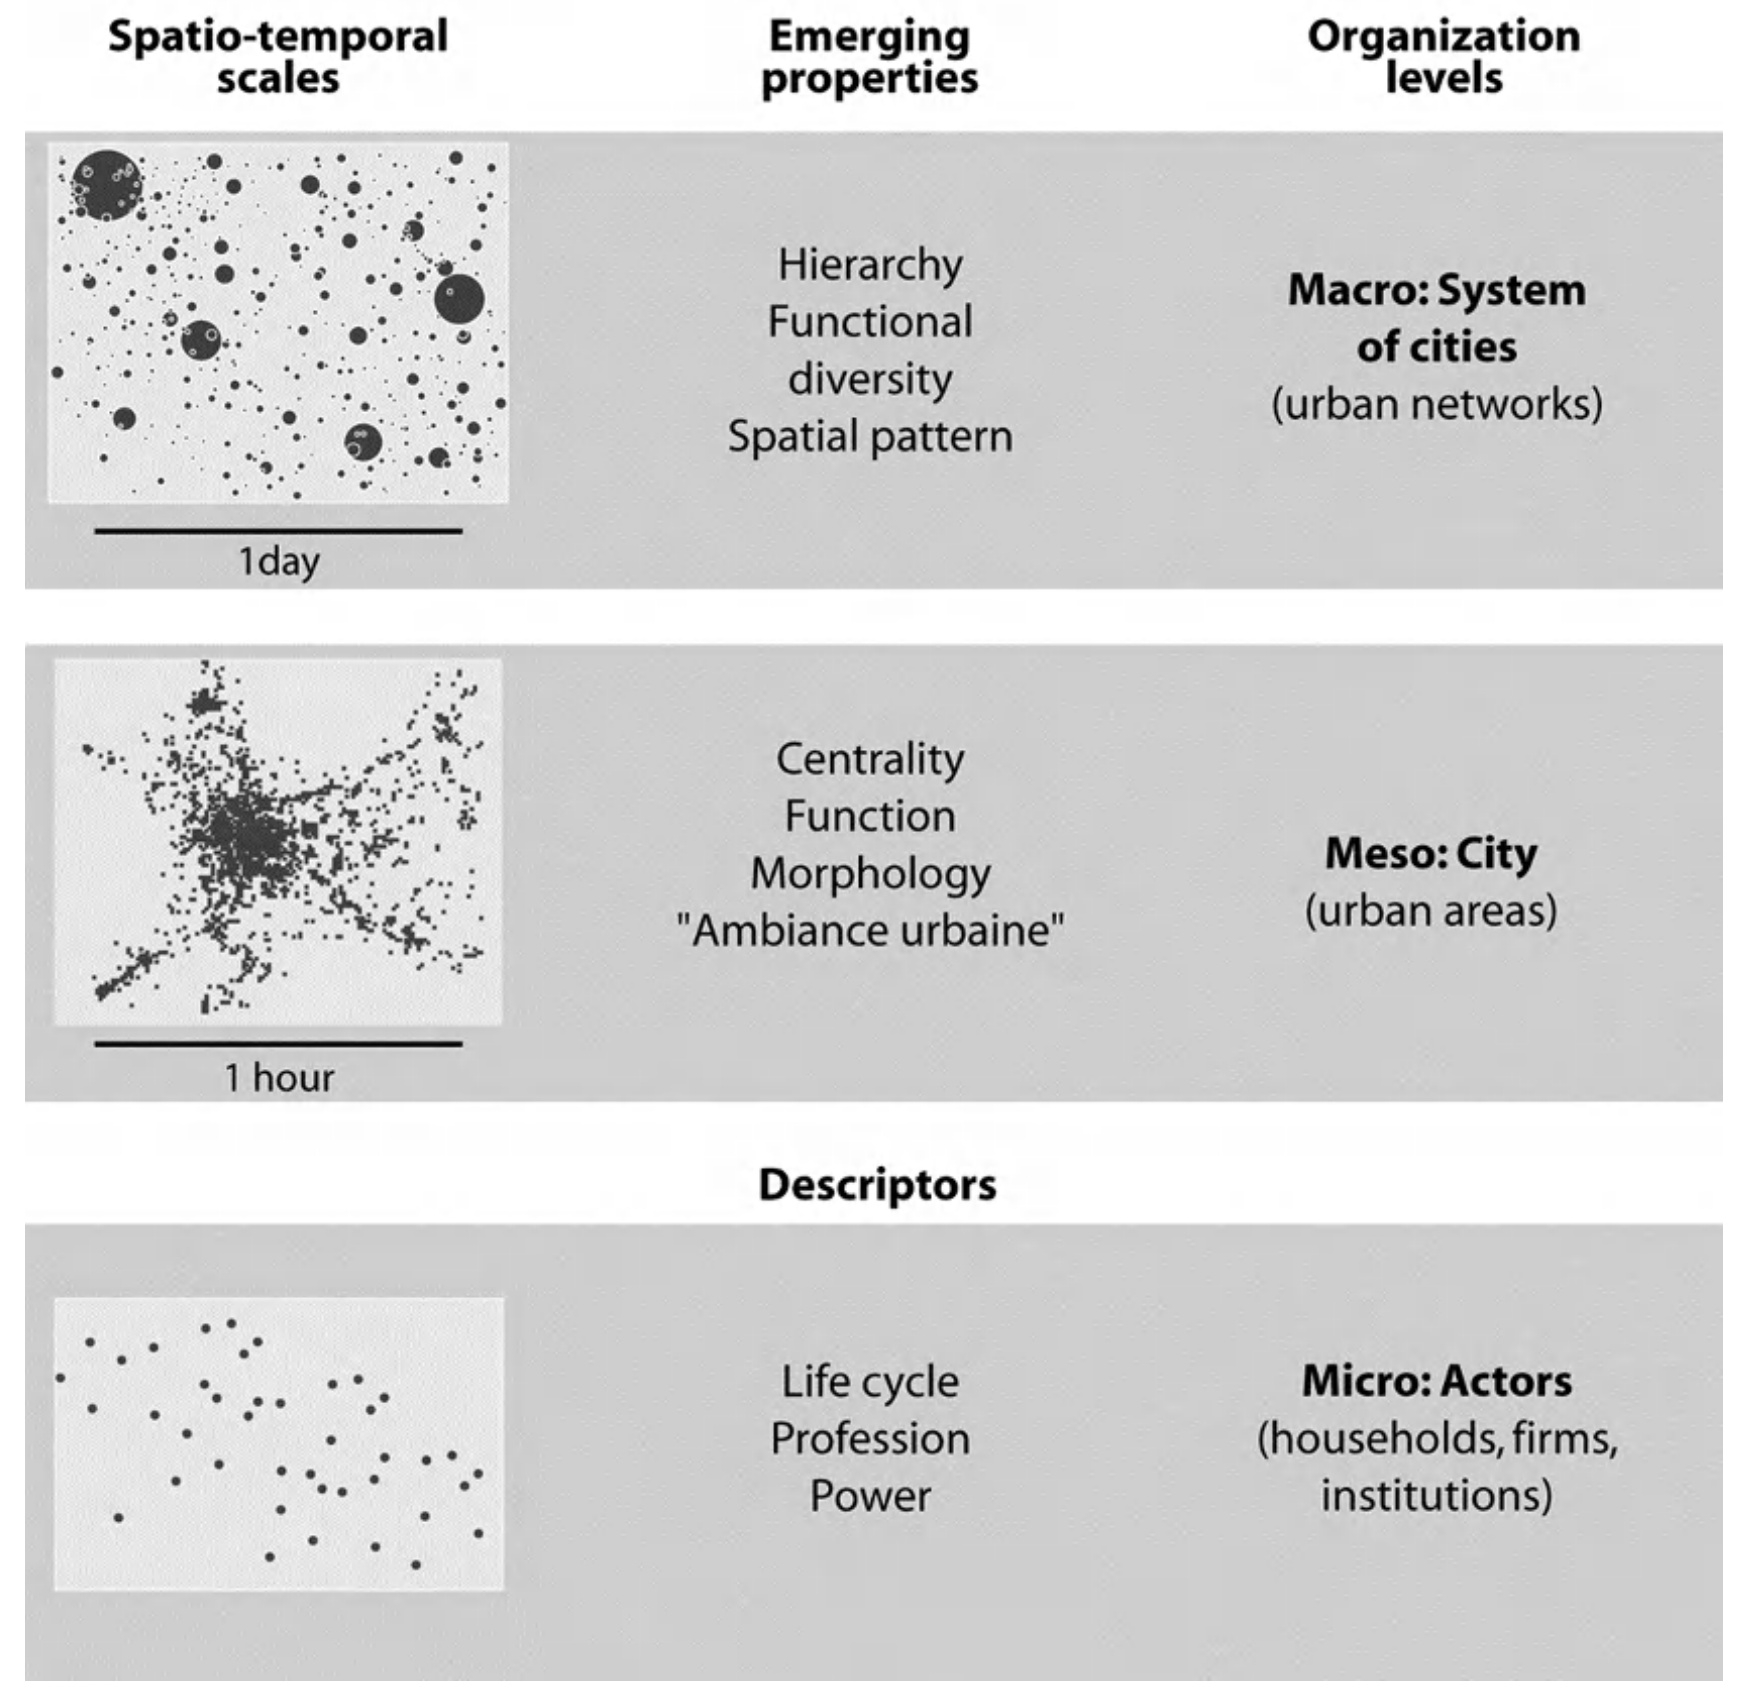
\includegraphics[width=0.9\textwidth]{../../../Communications/ALife2020/figures/evoltheory_scales.png}
	\end{column}
	\begin{column}{0.3\linewidth}
	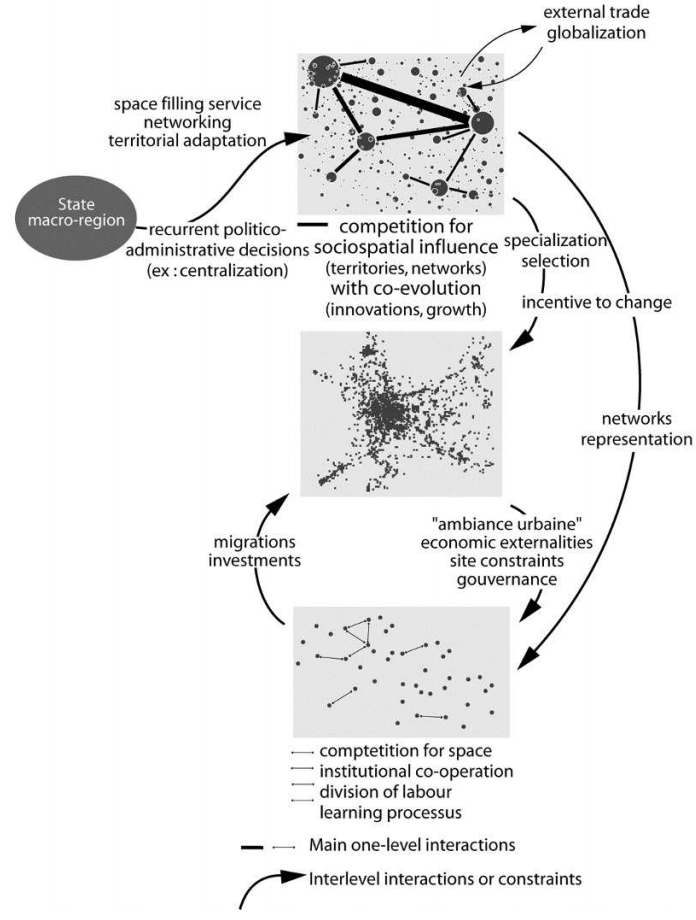
\includegraphics[width=\linewidth]{figures/evolth_feedbacks.png}
	
	\end{column}
	\end{columns}
\end{center}

\footnotesize
\textit{An evolutionary urban theory considering cities as systems within systems of cities; co-evolving urban systems in which interactions are crucial \cite{pumain2018evolutionary} \cite{pumain1997pour} \cite{pumain2008socio}}

}


\sframe{The series of Simpop models \cite{pumain2012multi}}{

\begin{columns}

	\begin{column}{0.5\textwidth}
	
	\centering
	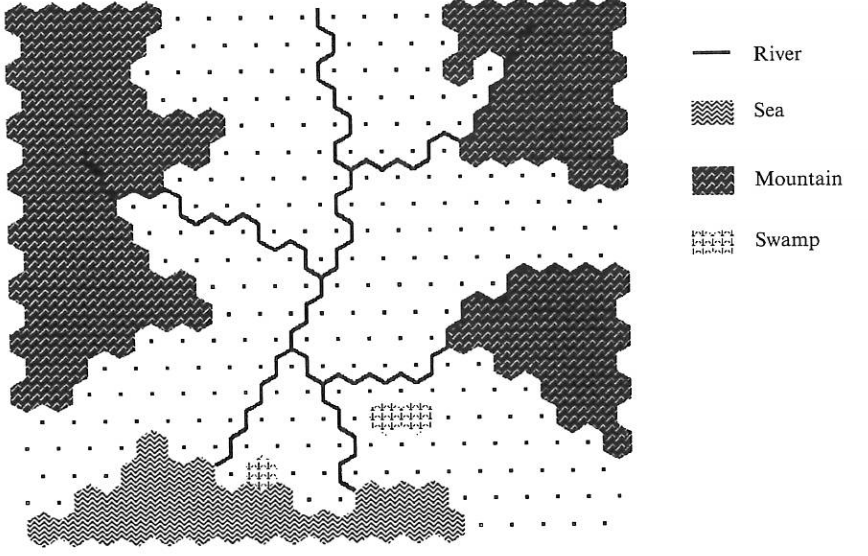
\includegraphics[width=0.75\textwidth]{../../../../../OpenMole/courses/spatialsens/figures/simpop1.png}
	
	\footnotesize
\textit{Simpop 1 model \cite{sanders1997simpop}}

	\medskip
	\hrule
	\centering
	
	\medskip
	
	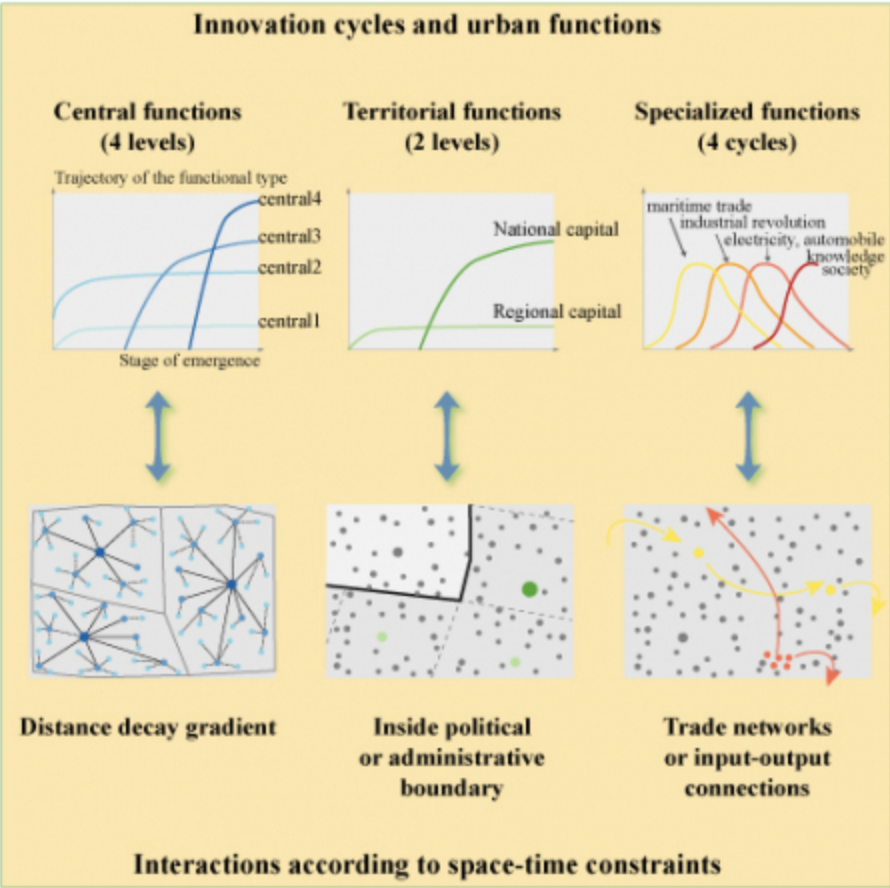
\includegraphics[width=0.55\textwidth,height=0.3\textheight]{figures/simpop2.png}
	
	\footnotesize
	
	\textit{Simpop 2 model \cite{bretagnolle2006theory}}
	

	\end{column}
	\vrule{}
	\begin{column}{0.5\textwidth}
	
	
	
	\centering
	
	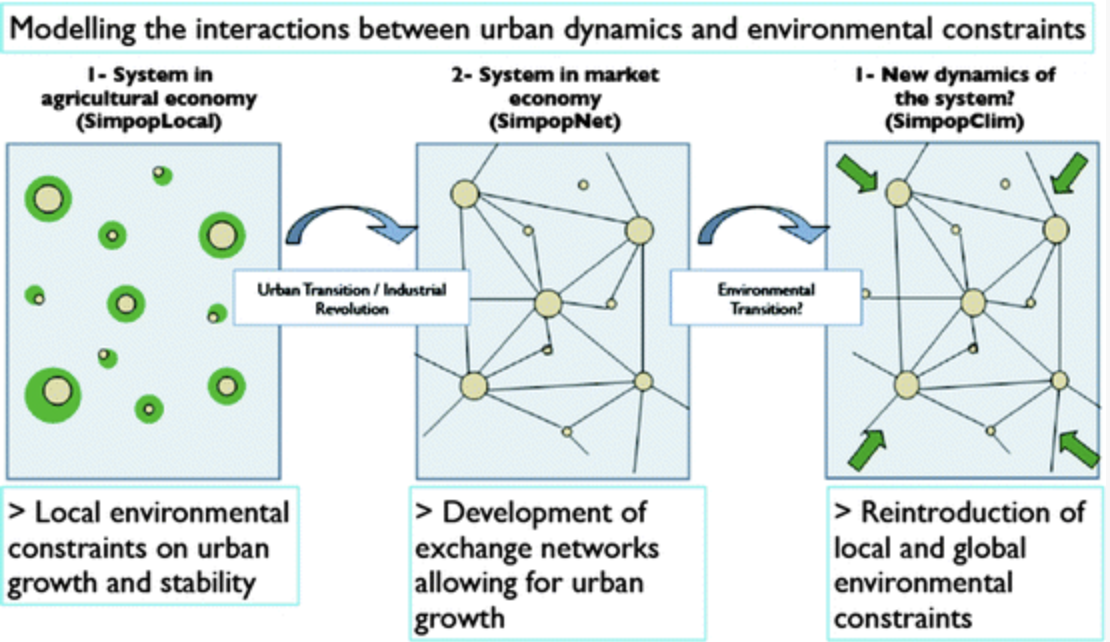
\includegraphics[width=0.9\textwidth]{figures/simpopseries.png}
	
	\footnotesize

	\textit{From SimpopLocal to SimpopClim \cite{pumain2012multi}}
	
	\medskip
	
	\hrule
	
	\medskip

	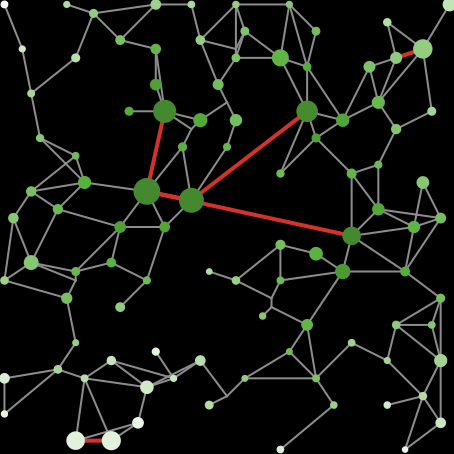
\includegraphics[width=0.5\textwidth]{../../../../../OpenMole/courses/spatialsens/figures/setup_synth_1_tick100.png}
	
	\footnotesize
	\textit{SimpopNet model \cite{schmitt2014modelisation}}
	
	\end{column}


\end{columns}

}


\sframe{Towards new practices: ERC Geodivercity}{

% presentation generale de Geodivercity

\begin{columns}
\begin{column}{0.4\textwidth}
	\centering
	\includegraphics[width=\textwidth]{../../../../../OpenMole/courses/spatialsens/figures/urban-dynamics-simulation-models-geodivercity.png}
\end{column}
\begin{column}{0.6\textwidth}

	$\rightarrow$ Recurrent stylized facts on main systems of cities
	
	$\rightarrow$ Construction of simulation models (with an explicative purpose)
	
	$\rightarrow$ Tools and methods to explore simulation models
	
	\bigskip
	
	%
\includegraphics[width=\textwidth]{../../../../../OpenMole/courses/spatialsens/figures/openmole.png}
	
\includegraphics[height=0.13\textheight]{../../../Communications/ALife2020/figures/iconOM.png}
	
\includegraphics[height=0.13\textheight]{../../../Communications/ALife2020/figures/openmole.png}
		
	
\end{column}
\end{columns}


}


\sframe{Theories and models}{

Historical succession of epistemologies in the case of systems of cities
\cite{varenne2018theories}: 

\medskip

\begin{enumerate}
    \item Deduction from theory (top-down): Christaller
	\item Induction from the empirical (bottom-up): Berry
	\item Towards an abductive epistemology (iterative interaction theoretical-empirical): Pumain
\end{enumerate}

\medskip

$\rightarrow$ simulation allows synthesis

}


\sframe{Geographical systems and complexity}{

\textit{Necessity of simulation models in geography induced by complexities of these systems ?}

\bigskip

\begin{itemize}
	\item Ontological complexity \cite{pumain2003approche}
	\item Dynamical complexity: non-ergodicity and path-dependency \cite{pumain2012urban}
	\item Complexity and co-evolution \cite{raimbault2019modeling}
	\item Complexity and emergence \cite{bedau2002downward}
\end{itemize}

}


\sframe{Construction of Knowledge across Domains}{

\centering

\includegraphics[height=0.9\textheight]{../../../../../OpenMole/courses/spatialsens/figures/openmoleslide}


\nocite{baffi:tel-01389347}
\nocite{pumain2008socio}
\nocite{reuillon2013openmole}
\nocite{cottineau2015modular}
\nocite{swerts2017database}
\nocite{pumain1997pour}
\nocite{pumain2010theorie}

}

\sframe{Bibliometrics of the Evolutionary Urban Theory}{

\begin{center}
\includegraphics[height=0.7\textheight]{../../../../../OpenMole/courses/spatialsens/figures/evolurbantheory.pdf}
\end{center}

\textit{Citation network analysis of key publications}

\smallskip

\footnotesize
Raimbault, J. (2017). An Applied Knowledge Framework to Study Complex Systems. In Complex Systems Design \& Management (pp. 31-45).

\nocite{raimbault2017applied}


}






\sframe{OpenMOLE software}{

\justify


Urban simulation models integrated into the OpenMOLE open source software for model exploration and validation

\begin{center}

\includegraphics[height=0.13\textheight]{../../../Communications/ALife2020/figures/iconOM.png}

\includegraphics[height=0.13\textheight]{../../../Communications/ALife2020/figures/openmole.png}
\end{center}


\textit{Enables seamlessly (i) model embedding; (ii) access to HPC resources; (iii) exploration and optimization algorithms}

\medskip

\url{https://openmole.org/}

\medskip

\textbf{Applications for the summer school} (May 30th-June 4th 2021) are open!  \url{https://exmodelo.org/}

\medskip

\footnotesize

Reuillon, R., Leclaire, M., \& Rey-Coyrehourcq, S. (2013). OpenMOLE, a workflow engine specifically tailored for the distributed exploration of simulation models. Future Generation Computer Systems, 29(8), 1981-1990.

\nocite{reuillon2013openmole}

}




\sframe{Calibration of SimpopLocal model}{

\footnotesize
\textit{SimpopLocal model calibrated with distributed NSGA2 on grid}

%\medskip
%Formalising the expectations
%\textit{Formalising the expectations as indicators: }

\begin{center}
	\includegraphics[width=0.8\textwidth]{../../../../../OpenMole/courses/spatialsens/figures/slocal_fitness.png}
\end{center}
	
\smallskip

\tiny

Schmitt, C., Rey-Coyrehourcq, S., Reuillon, R., \& Pumain, D. (2015). Half a billion simulations: Evolutionary algorithms and distributed computing for calibrating the SimpopLocal geographical model. Environment and Planning B: Planning and Design, 42(2), 300-315.

\nocite{schmitt2015half}

}

\sframe{SimpopLocal and calibration profile}{

\textit{Computes the best calibration at fixed steps along one dimension.}
 
 \medskip
 
 \includegraphics[width=0.48\textwidth]{../../../../../OpenMole/courses/spatialsens/figures/PdiffusionZ.png}
 \includegraphics[width=0.48\textwidth]{../../../../../OpenMole/courses/spatialsens/figures/InnovationLife.png}
 
 \bigskip
 
 \footnotesize

Reuillon, R., Schmitt, C., De Aldama, R., \& Mouret, J. B. (2015). A new method to evaluate simulation models: the calibration profile (cp) algorithm. Journal of Artificial Societies and Social Simulation, 18(1), 12.

 \nocite{reuillon2015new}

}


\sframe{Unicity of mechanisms: multi-modeling}{

\footnotesize
\textit{Automate the confrontation of alternative hypothesis / mechanisms}

\medskip

	
	\begin{center}
	\includegraphics[width=0.9\textwidth]{../../../../../OpenMole/courses/spatialsens/figures/simfamily.png}
	\end{center}
	
\tiny

Cottineau, C., Reuillon, R., Chapron, P., Rey-Coyrehourcq, S., \& Pumain, D. (2015). A modular modelling framework for hypotheses testing in the simulation of urbanisation. Systems, 3(4), 348-377.

\nocite{cottineau2015modular}

}

\sframe{Multi-modeling (64 models)}{

%64 models

\centering

\includegraphics[width=0.6\textwidth]{../../../../../OpenMole/courses/spatialsens/figures/marius_complexification.png}


}


\sframe{Exemple of concurrent hypothesis}{


%Exchange mechanism:

%Market based
%Centrally planned

\textbf{Exchange mechanism: } market vs centralized

\medskip

%City growth mechanism:
%Purely inter-urban interactions
%Influenced by environmental situation

\textbf{City growth: } interurban interactions vs environmental situation

\bigskip
\bigskip

\centering

\includegraphics[width=0.5\textwidth]{../../../../../OpenMole/courses/spatialsens/figures/system_mec.png}

}


\sframe{Calibration of model family}{

%
\textit{Compute the best set of parameters for all 64 models.}

\bigskip

\centering

\includegraphics[width=\textwidth]{../../../../../OpenMole/courses/spatialsens/figures/varius_big.png}

% http://shiny.parisgeo.cnrs.fr/VARIUS/

}




\sframe{Other example of multi-modeling}{

%\textit{Benchmark of growth models for systems of cities}

\begin{center}
\includegraphics[width=0.8\textwidth]{../../../../../UrbanGrowth/Docs/Papers/EvolutionaryTheory/paper/figures/Fig5}
\end{center}

\footnotesize

Raimbault, J.; Denis, E.; Pumain, D. (2020). Empowering Urban Governance through Urban Science: Multi-Scale Dynamics of Urban Systems Worldwide. Sustainability 2020, 12, 5954.



\nocite{Raimbault_2020}



}






\sframe{PSE algorithm on the MARIUS model}{

\textit{Diversity of urban systems dynamics produced by the MARIUS model} 


\begin{center}
\includegraphics[width=0.5\textwidth]{../../../../../OpenMole/courses/spatialsens/figures/pse_marius.png}
\end{center}

\footnotesize

Chérel, G., Cottineau, C., \& Reuillon, R. (2015). Beyond corroboration: Strengthening model validation by looking for unexpected patterns. PloS one, 10(9), e0138212.

\nocite{10.1371/journal.pone.0138212}

}




\sframe{Spatial sensitivity analysis}{

% space matters

\begin{center}
	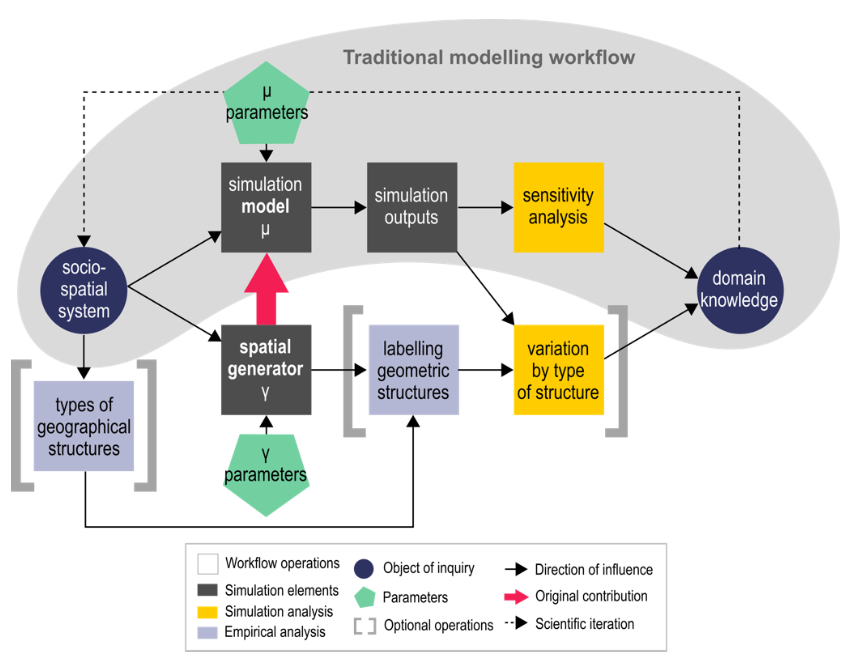
\includegraphics[width=0.7\linewidth]{figures/spacematters.png}
\end{center}

\medskip

\tiny

Raimbault, J., Cottineau, C., Le Texier, M., Le Nechet, F., \& Reuillon, R. (2019). Space Matters: Extending Sensitivity Analysis to Initial Spatial Conditions in Geosimulation Models. Journal of Artificial Societies and Social Simulation, 22(4).

\nocite{raimbault2019space}


}

\sframe{Spatial sensitivity analysis: synthetic data}{

% spatial synthetic data

\begin{center}
	\includegraphics[width=0.28\linewidth]{../../../../../UrbanDynamics/Docs/Seminars/20201007_CasaST/synthdata.jpg}\hspace{0.2cm}
	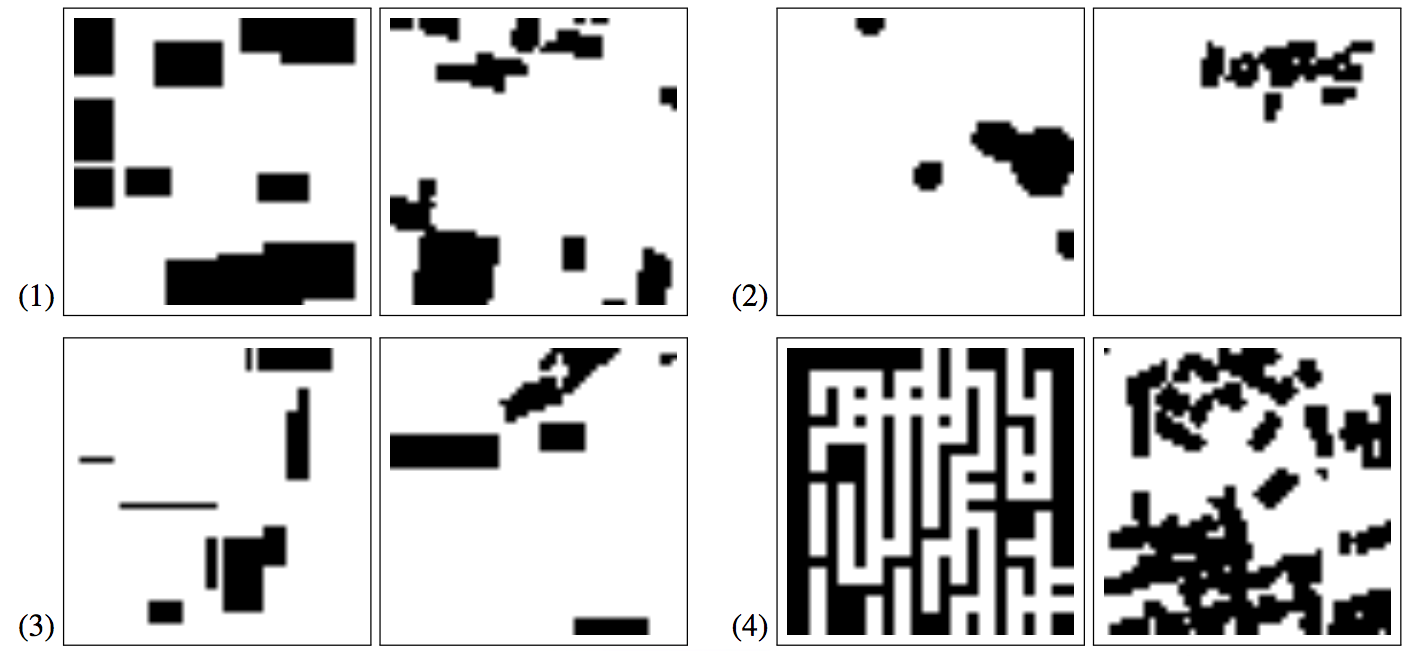
\includegraphics[width=0.6\linewidth]{../../../../../UrbanDynamics/Docs/Seminars/20201007_CasaST/spatialsens_calib.png}
\end{center}

\bigskip

\footnotesize


Raimbault, J. (2019). Second-order control of complex systems with correlated synthetic data. Complex Adaptive Systems Modeling, 7(1), 1-19.
\nocite{raimbault2019second}

\medskip

Raimbault, J., \& Perret, J. (2019). Generating urban morphologies at large scales. In Artificial Life Conference Proceedings (pp. 179-186).
\nocite{raimbault2019generating}


}







\section{A model of urban evolution based on innovation diffusion}



% We then describe a model of urban evolution positioned in this approach, in which the diffusion of innovations between cities captures transformation processes (mutations) and transmission processes (diffusion), using two coupled spatial interaction models. Explorations of the model on synthetic systems of cities show the role of spatial interaction and innovation diffusion ranges on measures of diversity and utility, and the existence of intermediate interaction ranges yielding an optimal util- ity. Multi-objective optimization shows how the model produces a compromise between utility and diversity.


\sframe{Innovation diffusion}{


%\justify

$\rightarrow$ \textbf{Innovation diffusion} is a crucial process in artificial life evolutionary systems and open-ended evolution \cite{bedau2000open}

\medskip

$\rightarrow$ Artificial societies used to study the dynamics of innovation \cite{zenobia2009artificial}

\medskip

$\rightarrow$ Innovations diffuse hierarchically in systems of cities \cite{hagerstrand1968innovation}, potential explanation of urban scaling laws \cite{pumain2006evolutionary}

\bigskip

\textit{Innovation diffusion as a privileged entry to understand urban evolution}


}


\sframe{Model objective}{


$\rightarrow$ Concepts of urban evolution do not necessarily capture essential processes (transmission and transformation) in the literature

\medskip

$\rightarrow$ Need for simple models with explicit urban genome at the system of cities scale


\bigskip

\textbf{Research objective: }

\medskip

\textit{Describe and systematically explore an urban evolution model based on innovation diffusion, for urban dynamics at the macroscopic scale}

\bigskip
\bigskip

\footnotesize

Raimbault, J. (2020). A model of urban evolution based on innovation diffusion. Artificial Life Conference Proceedings 2020 NO. 32, 500-508.



}



\sframe{Model rationale}{

\begin{itemize}
	\item Agents are cities, macroscopic scale (regional, country, continental) and long time scales (century)
	\item Cities characterized by their size in terms of population; genome as adoption proportions of innovations (social or technological) for each city (one single dimension to simplify)
	\item Following \cite{favaro2011gibrat}, attractivity of cities due to level of innovation drive their population growth through spatial interactions; innovation diffuse through an other spatial interaction model \cite{fotheringham1989spatial}
	\item Mutations occur in cities as new innovations appear
\end{itemize}


}



\sframe{Model description}{

% step by step scheme ?


\begin{pspicture}(0,-2.94)(11.17,2.94)
\definecolor{colour0}{rgb}{1.0,0.2,0.0}
\definecolor{colour1}{rgb}{0.2,0.8,0.0}
\definecolor{colour2}{rgb}{0.0,0.8,1.0}
\pscircle[linecolor=black, linewidth=0.04, dimen=outer](0.8,0.26){0.8}
\pscircle[linecolor=black, linewidth=0.04, dimen=outer](3.44,-1.9){0.38}
\pscircle[linecolor=black, linewidth=0.04, dimen=outer](4.64,2.08){0.5}
\pscircle[linecolor=black, linewidth=0.04, dimen=outer](6.72,-2.12){0.48}
\rput[bl](0.12,1.1){\textit{City 1}}
\rput[bl](4.16,2.64){\textit{City 2}}
\rput[bl](2.88,-2.66){\textit{City 3}}
\rput[bl](6.16,-2.94){\textit{City 4}}
\pscircle[linecolor=black, linewidth=0.04, dimen=outer](7.56,2.48){0.44}
\pscircle[linecolor=black, linewidth=0.04, dimen=outer](7.56,2.38){0.34}
\pscircle[linecolor=black, linewidth=0.04, dimen=outer](7.56,2.28){0.22}
\rput[bl](8.18,2.18){Population}
\psframe[linecolor=black, linewidth=0.04, fillstyle=solid,fillcolor=colour0, dimen=outer](7.66,1.56)(7.4,1.22)
\psframe[linecolor=black, linewidth=0.04, fillstyle=solid,fillcolor=colour1, dimen=outer](7.66,1.74)(7.4,1.54)
\psframe[linecolor=black, linewidth=0.04, fillstyle=solid,fillcolor=colour2, dimen=outer](7.66,1.94)(7.4,1.72)
\rput[bl](8.14,1.46){Innovation genome}
\psframe[linecolor=black, linewidth=0.04, fillstyle=solid,fillcolor=colour0, dimen=outer](0.82,0.2)(0.56,-0.38)
\psframe[linecolor=black, linewidth=0.04, fillstyle=solid,fillcolor=colour0, dimen=outer](4.72,2.2)(4.52,1.72)
\psframe[linecolor=black, linewidth=0.04, fillstyle=solid,fillcolor=colour0, dimen=outer](6.74,-1.94)(6.54,-2.44)
\psframe[linecolor=black, linewidth=0.04, fillstyle=solid,fillcolor=colour0, dimen=outer](3.48,-1.8)(3.3,-2.16)
\psframe[linecolor=black, linewidth=0.04, fillstyle=solid,fillcolor=colour1, dimen=outer](0.82,0.58)(0.56,0.18)
\only<2->{
\psframe[linecolor=black, linewidth=0.04, fillstyle=solid,fillcolor=colour1, dimen=outer](4.72,2.4)(4.52,2.18)
\psframe[linecolor=black, linewidth=0.04, fillstyle=solid,fillcolor=colour1, dimen=outer](3.48,-1.6)(3.3,-1.82)
\psframe[linecolor=black, linewidth=0.04, fillstyle=solid,fillcolor=colour1, dimen=outer](6.74,-1.76)(6.54,-1.98)
\psline[linecolor=colour1, linewidth=0.04, linestyle=dashed, dash=0.17638889cm 0.10583334cm, arrowsize=0.05291667cm 2.0,arrowlength=1.4,arrowinset=0.0]{<-}(4.08,2.08)(1.4,0.84)
\psline[linecolor=colour1, linewidth=0.04, linestyle=dashed, dash=0.17638889cm 0.10583334cm, arrowsize=0.05291667cm 2.0,arrowlength=1.4,arrowinset=0.0]{<-}(6.16,-2.1)(1.48,-0.14)
\psline[linecolor=colour1, linewidth=0.04, linestyle=dashed, dash=0.17638889cm 0.10583334cm, arrowsize=0.05291667cm 2.0,arrowlength=1.4,arrowinset=0.0]{<-}(3.06,-1.74)(1.2,-0.44)
\psline[linecolor=colour1, linewidth=0.04, linestyle=dashed, dash=0.17638889cm 0.10583334cm, arrowsize=0.05291667cm 2.0,arrowlength=1.4,arrowinset=0.0]{<-}(7.98,0.5)(7.1,0.5)
\rput[bl](8.14,0.4){Innovation diffusion}
}
\only<3->{
\psline[linecolor=black, linewidth=0.08, arrowsize=0.05291667cm 2.0,arrowlength=1.4,arrowinset=0.0]{<->}(1.56,0.5)(4.18,1.74)
\psline[linecolor=black, linewidth=0.16, arrowsize=0.05291667cm 2.0,arrowlength=1.4,arrowinset=0.0]{<->}(1.6,0.04)(6.2,-1.88)
\psline[linecolor=black, linewidth=0.08, arrowsize=0.05291667cm 2.0,arrowlength=1.4,arrowinset=0.0]{<->}(4.88,1.62)(6.46,-1.6)
\psline[linecolor=black, linewidth=0.04, arrowsize=0.05291667cm 2.0,arrowlength=1.4,arrowinset=0.0]{<->}(1.44,-0.32)(3.16,-1.54)
\psline[linecolor=black, linewidth=0.04, arrowsize=0.05291667cm 2.0,arrowlength=1.4,arrowinset=0.0]{<->}(3.86,-1.94)(6.2,-2.22)
\psline[linecolor=black, linewidth=0.04, arrowsize=0.05291667cm 2.0,arrowlength=1.4,arrowinset=0.0]{<->}(7.06,0.96)(7.96,0.96)
\psline[linecolor=black, linewidth=0.08, arrowsize=0.05291667cm 2.0,arrowlength=1.4,arrowinset=0.0]{<->}(3.7,-1.5)(4.62,1.5)
\rput[bl](8.12,0.84){Population growth}
}
\only<4->{
\psframe[linecolor=black, linewidth=0.04, fillstyle=solid,fillcolor=colour2, dimen=outer](0.82,0.94)(0.56,0.56)
\pscircle[linecolor=colour2, linewidth=0.04, linestyle=dashed, dash=0.17638889cm 0.10583334cm, dimen=outer](0.81,0.27){0.72}
\pscircle[linecolor=colour2, linewidth=0.04, linestyle=dashed, dash=0.17638889cm 0.10583334cm, dimen=outer](7.6,-0.08){0.26}
\rput[bl](8.14,-0.18){Mutation}
}
\end{pspicture}



}


\sframe{Model formalization}{

\footnotesize

At each time step, with $P_i \left(t\right)$ population, $\delta_{c,i}\left(t\right)$ genome, $u_c$ utility of innovation, $p_{c,i,t}$ share of total population adopting innovation $c$ in city $i$
\begin{enumerate}
	\item Crossover through the diffusion of innovations
	\[
	\delta_{c,i,t} \textrm{ = } \frac{\sum_j p_{c,j,t-1}^{\frac{1}{u_c}} \cdot \exp{\left(-\frac{d_{ij}}{d_I}\right)}}{\sum_c \sum_j p_{c,j,t-1}^{\frac{1}{u_c}} \cdot \exp{\left(-\frac{d_{ij}}{d_I}\right)}}	
	\]
	\item Population growth through spatial interactions $P_i\left(t\right) - P_i\left(t-1\right) \textrm{ = } w_I\cdot \sum_j \frac{V_{ij}}{<V_{ij}>}$ with
	\[ 
	V_{ij} \textrm{ = } \frac{P_{i}\left(t-1\right) \cdot P_{j}\left(t-1\right)}{\left(\sum_k P_k\left(t-1\right)\right)^2} \cdot \exp{\left(-\frac{d_{ij}}{d_G} \cdot \prod_c \delta_{c,i,t}^{\phi_{c,t}}\right)}
	\]
	and $\phi_{c,t} \textrm{ = } \sum_i \delta_{i,c,t}\cdot P_i\left(t-1\right) /\sum_{i,c} \delta_{i,c,t}\cdot P_{i}\left(t-1\right)$
	\item Mutations with innovations introduced with probability $\beta \cdot \left(P_i \left(t\right) / \max_k P_k \left(t\right)\right)^{\alpha_I}$ and an initial penetration rate $r_0$; new utility $u_c$ randomly distributed (normal or log-normal) with average current average utility and standard deviation a given parameter $\sigma_U$
\end{enumerate}



}


\sframe{Model indicators}{

\begin{itemize}
	\item Average diversity
	\[
	D \textrm{ = } \frac{1}{t_f \textrm{+} 1} \sum_{t\textrm{=}0}^{t_f} \left(1 - \sum_{i,c} \left(p_{c,i,t}\right)^2 \right)	
	\]
	\item Average utility
	\[
	U \textrm{ = } \frac{1}{t_f \textrm{ + } 1} \sum_{t \textrm{=}0}^{t_f} \sum_{i,c} \delta_{c,i,t} u_c 
	\]
	\item Innovatitivity 
	\[
	I \textrm{ = } \frac{\max c}{N\cdot \left(t_f \textrm{ + } 1\right)}
	\]
	\item Population trajectories, summarized by final hierarchy \cite{raimbault2020unveiling}
\end{itemize}



}



\sframe{Synthetic configurations}{

Model applied on synthetic systems of cities (so that conclusions are independent of geographical contingencies \cite{raimbault2019space}):

\medskip

\begin{itemize}
	\item random positions and rank-size hierarchy $P_i \left(0\right) \textrm{ = } \frac{P_{max}}{i^{\alpha_0}}$ with $\alpha_0 \textrm{ = } 1.0$ and $P_{max} \textrm{ = } 100,000$
	\item regional urban system scale: $N \textrm{ = } 30$ cities
	\item simulated for $t_f \textrm{ = } 50$ macroscopic time steps (order of magnitude of a century)
\end{itemize}



}



\sframe{Model parameters}{

\centering

	\begin{tabular}{|l|l|l|l|l|l|}
	\hline
	Parameter & Not. & Process & Range & Def. \\ \hline
	Number of cities & $N$ & Spatial scale & $[10 ; 100]$ & $30$\\
	Initial hierarchy & $\alpha_0$ & System of cities & $[0.5 ; 2.0]$ & $1$\\
	Initial population & $P_{max}$ & System of cities & $[10^4 ; 10^7]$ & $10^5$\\
	Simulation steps & $t_f$ & Temporal scale & $[10 ; 100]$ & $50$\\
	Growth rate & $w_I$ & Pop. growth & $[0.001 ; 0.01]$ & $0.005$\\\hline
	Gravity range & $d_G$ & Crossover & $[0 ; 2]$ & $1$\\
	Innovation range & $d_I$ & Crossover & $[0 ; 2]$ & $1$\\
	Innovation rate & $\beta$ & Mutation & $[0 ; 1]$ & $0.5$\\
	Innovation hierarchy & $\alpha_I$ & Mutation & $[0 ; 2]$ & $1$\\
	Innov. utility std. & $\sigma_U$ & Mutation & $\left[ 0.7;2\right]$ & $1$\\
	Penetration rate & $r_0$ & Mutation & $\left[0.1;0.9\right]$ & $0.5$\\
	Utility type & - & Mutation & \{n;ln\}& ln \\
	\hline
	\end{tabular}


% Model implemented in \texttt{scala}; relatively large parameter space


}




\sframe{Statistical consistency}{


\begin{itemize}
	\item Latin Hypercube Sampling of 100 parameter points, 1000 replications for each
	\item Sharpe ratios have high values for all indicators and all parameters (minimum 1.7 for utility)
	\item Average and median relative distances defined as $\Delta_{ij} \textrm{ = } 2\frac{\left|\mu_i - \mu_j \right|}{\sigma_i \textrm{ + } \sigma_j}$ larger than one for all indicators: 50 repetitions in further experiments
\end{itemize}




}


\sframe{Model exploration: diversity}{

Grid sampling of the parameter space (23,168 points, 50 replications) with a finer grid on $d_G$ and $d_I$; plots shown at $\alpha_I \textrm{ = } 1$ and $\sigma_U \textrm{ = } 1$

\medskip

\begin{center}
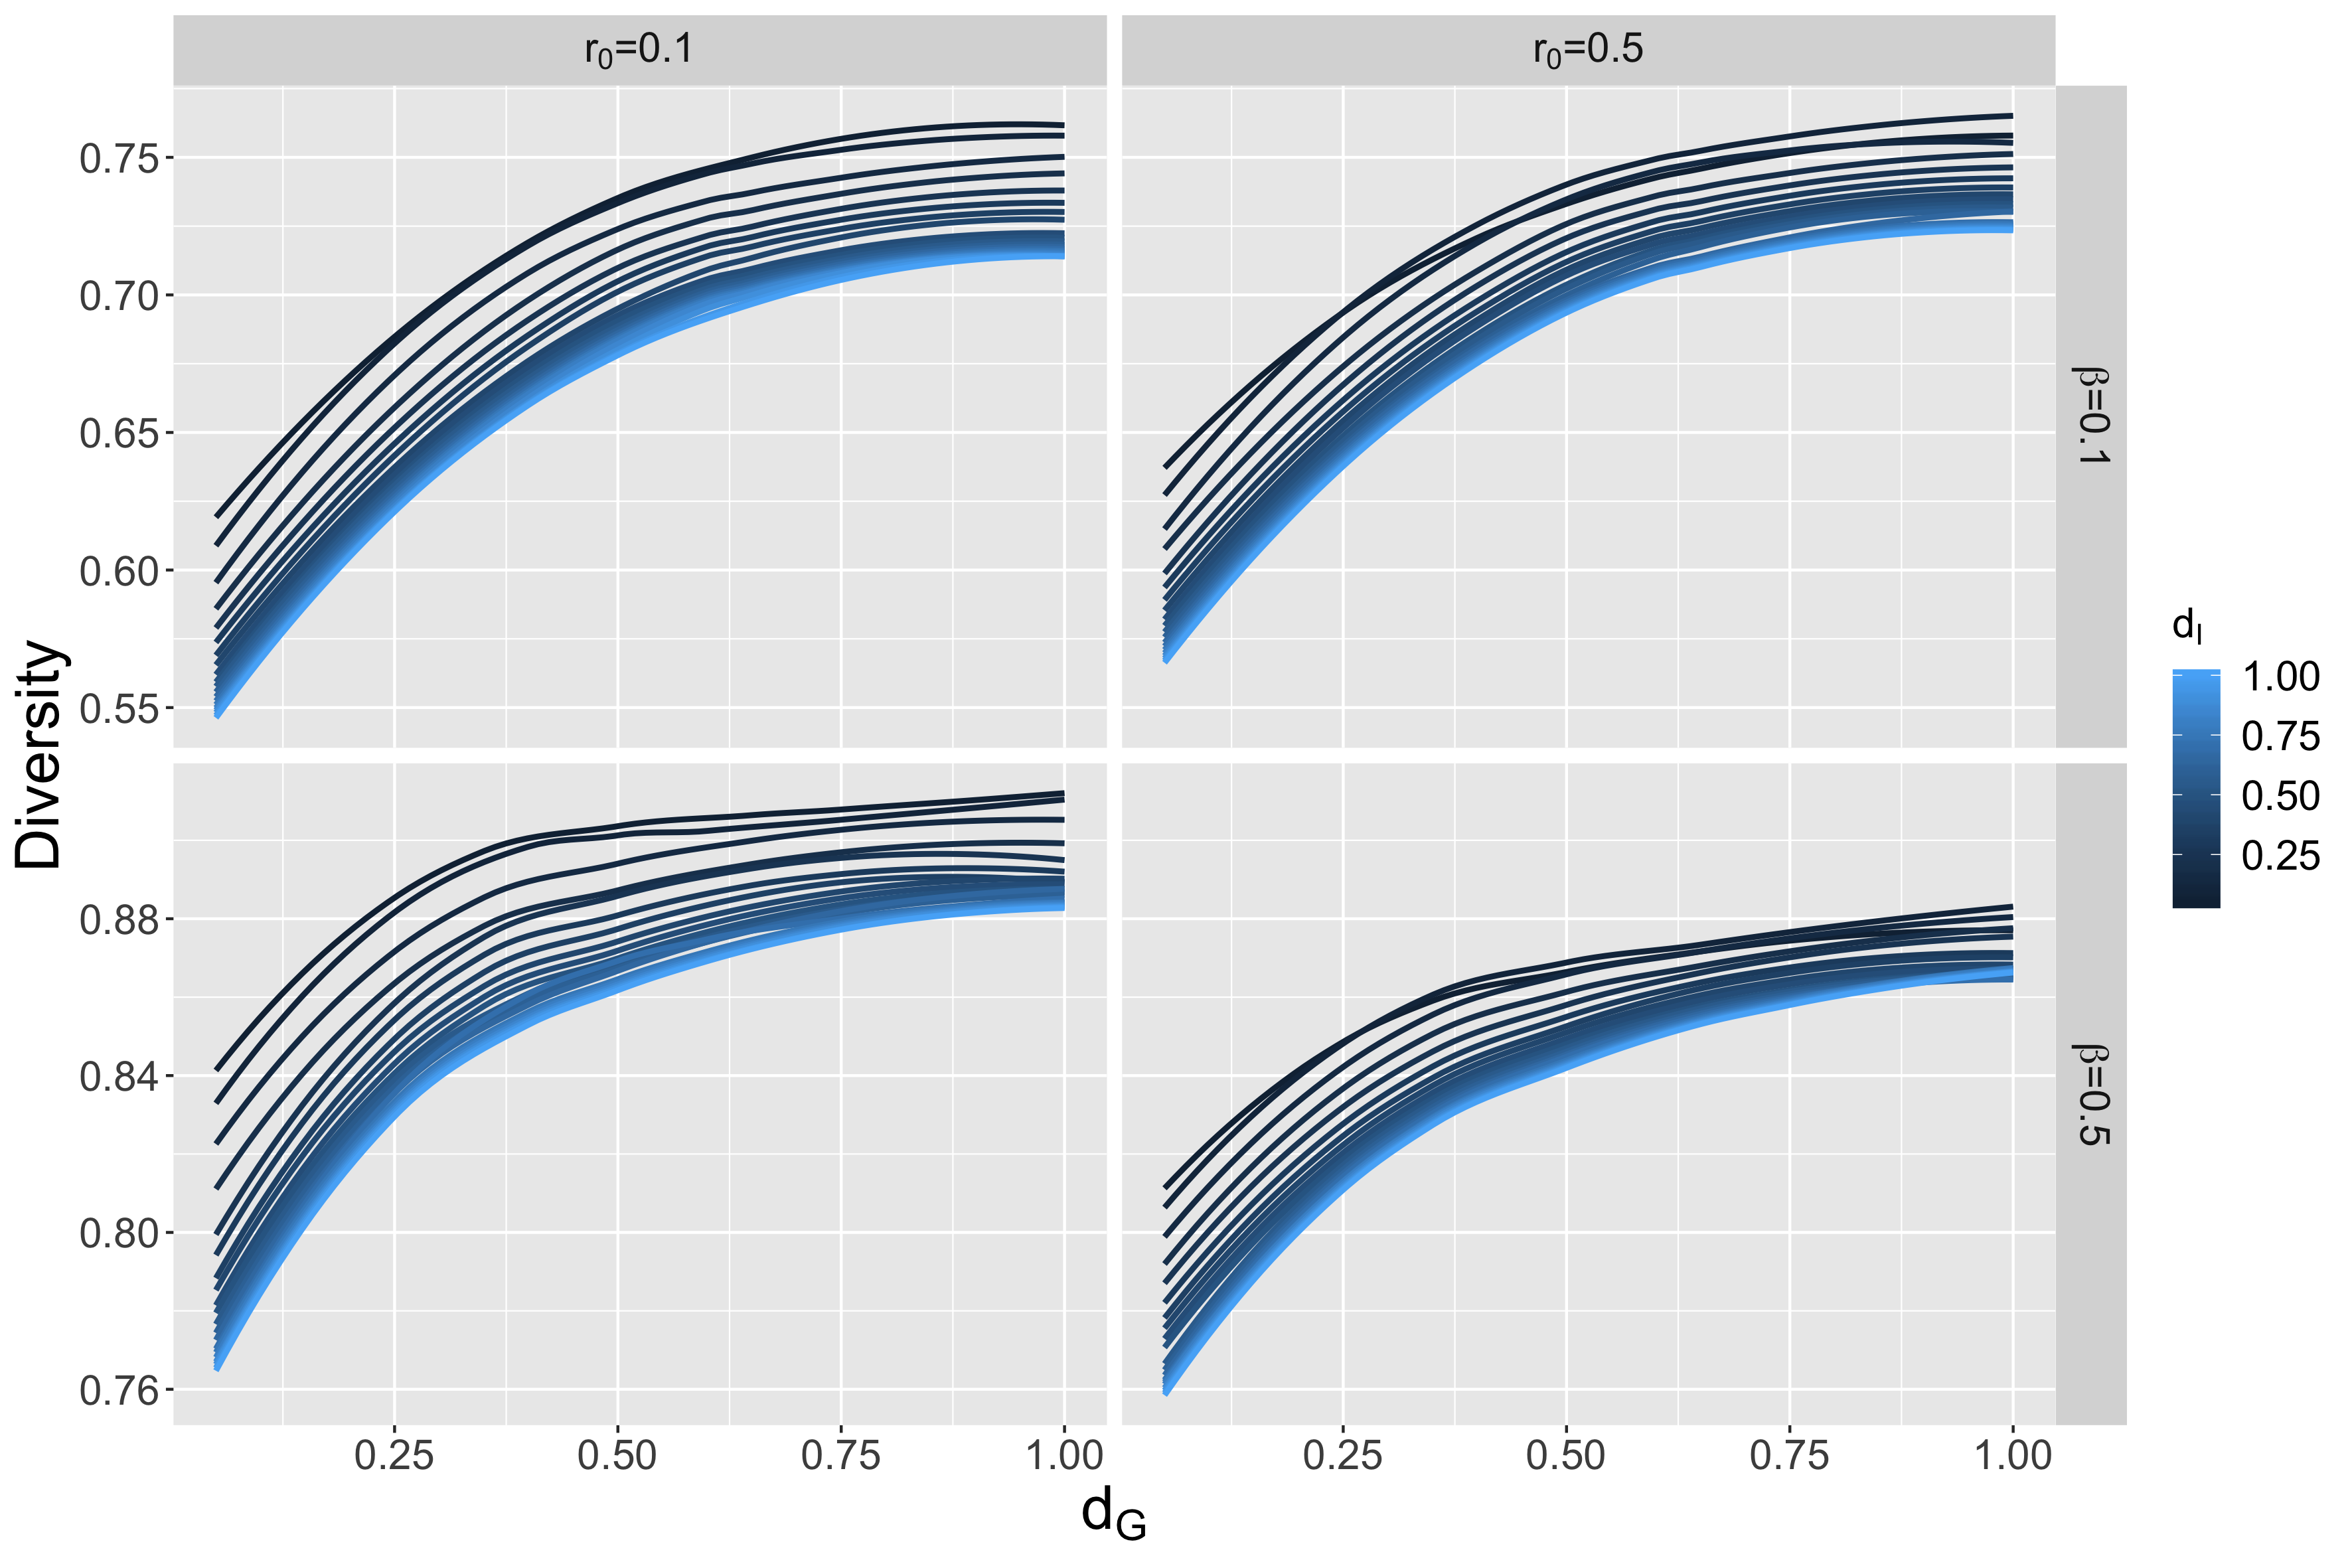
\includegraphics[width=0.7\linewidth]{../../../Communications/ALife2020/figures/averageDiversity-gravityDecay_color-innovationDecay_facet-mutationRate-earlyAdoptersRate_newInnovationHierarchy1_utilityStd1_distriblog-normal}
\end{center}

\smallskip

\footnotesize
\textit{Diversity increases with interaction span with a plateau behavior, decreases with innovation diffusion span}

}


\sframe{Model exploration: innovation and hierarchy}{

\begin{center}
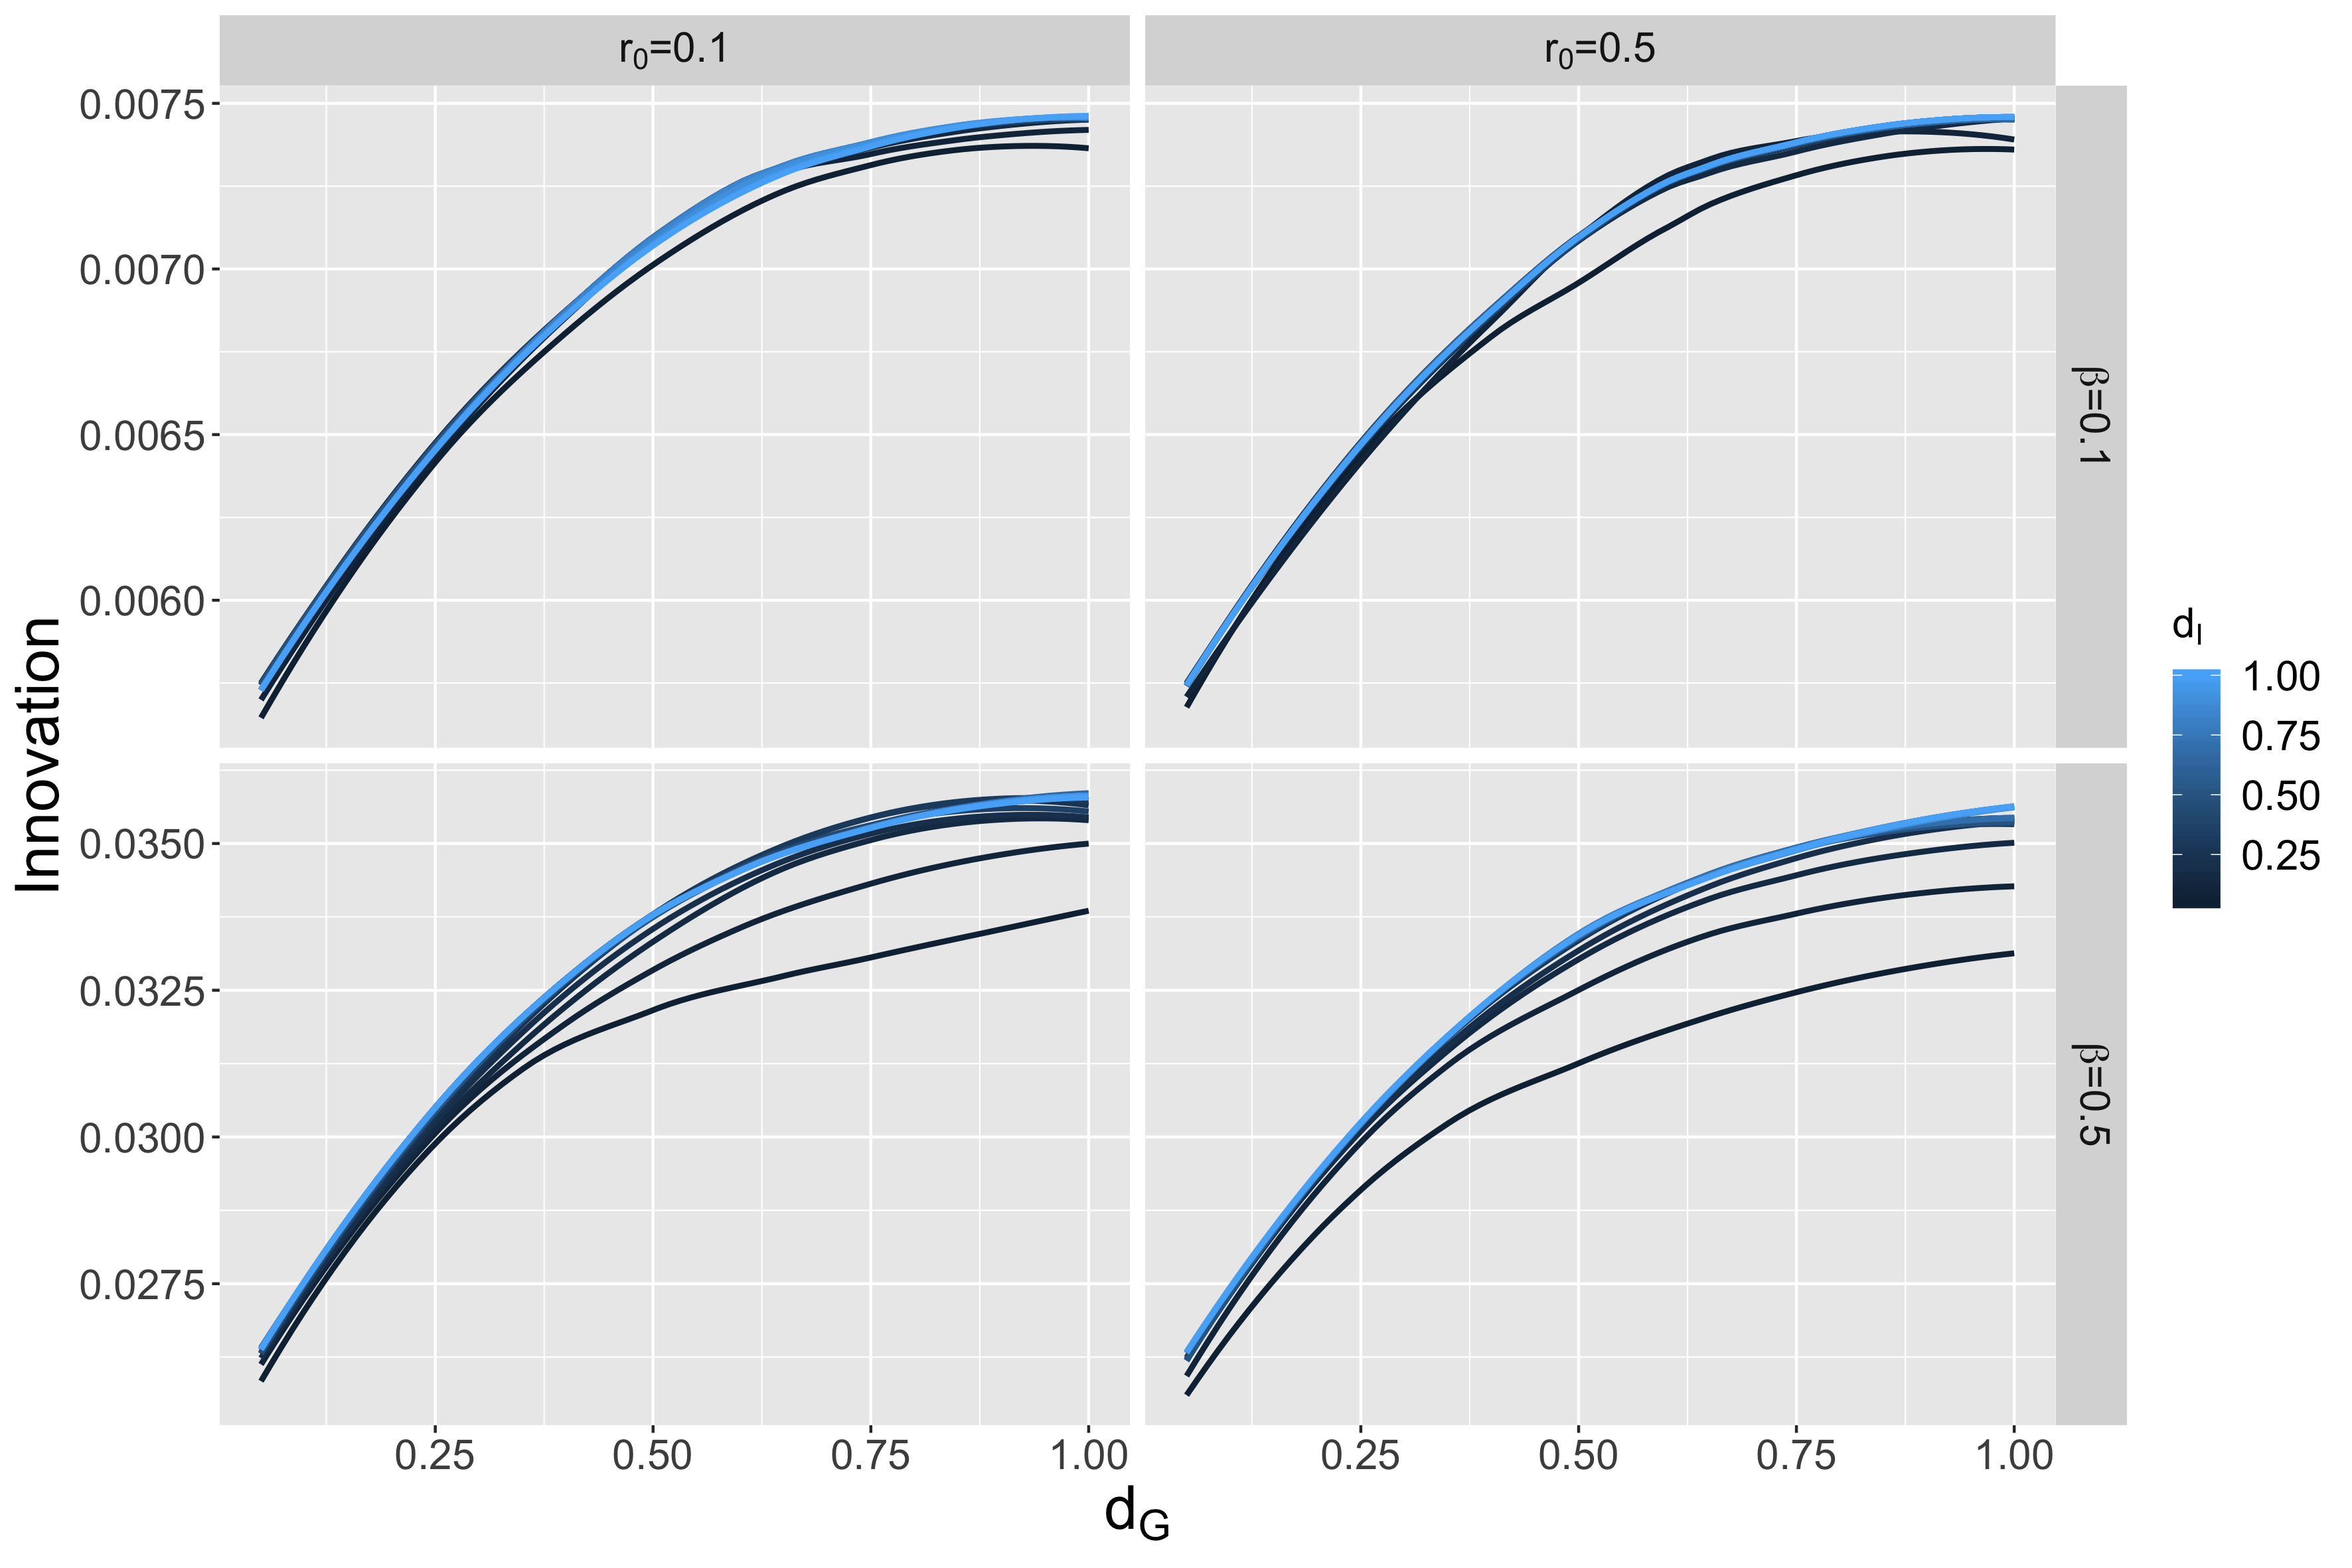
\includegraphics[width=0.47\linewidth]{../../../Communications/ALife2020/figures/averageInnovation-gravityDecay_color-innovationDecay_facet-mutationRate-earlyAdoptersRate_newInnovationHierarchy1_utilityStd1_distriblog-normal.png}
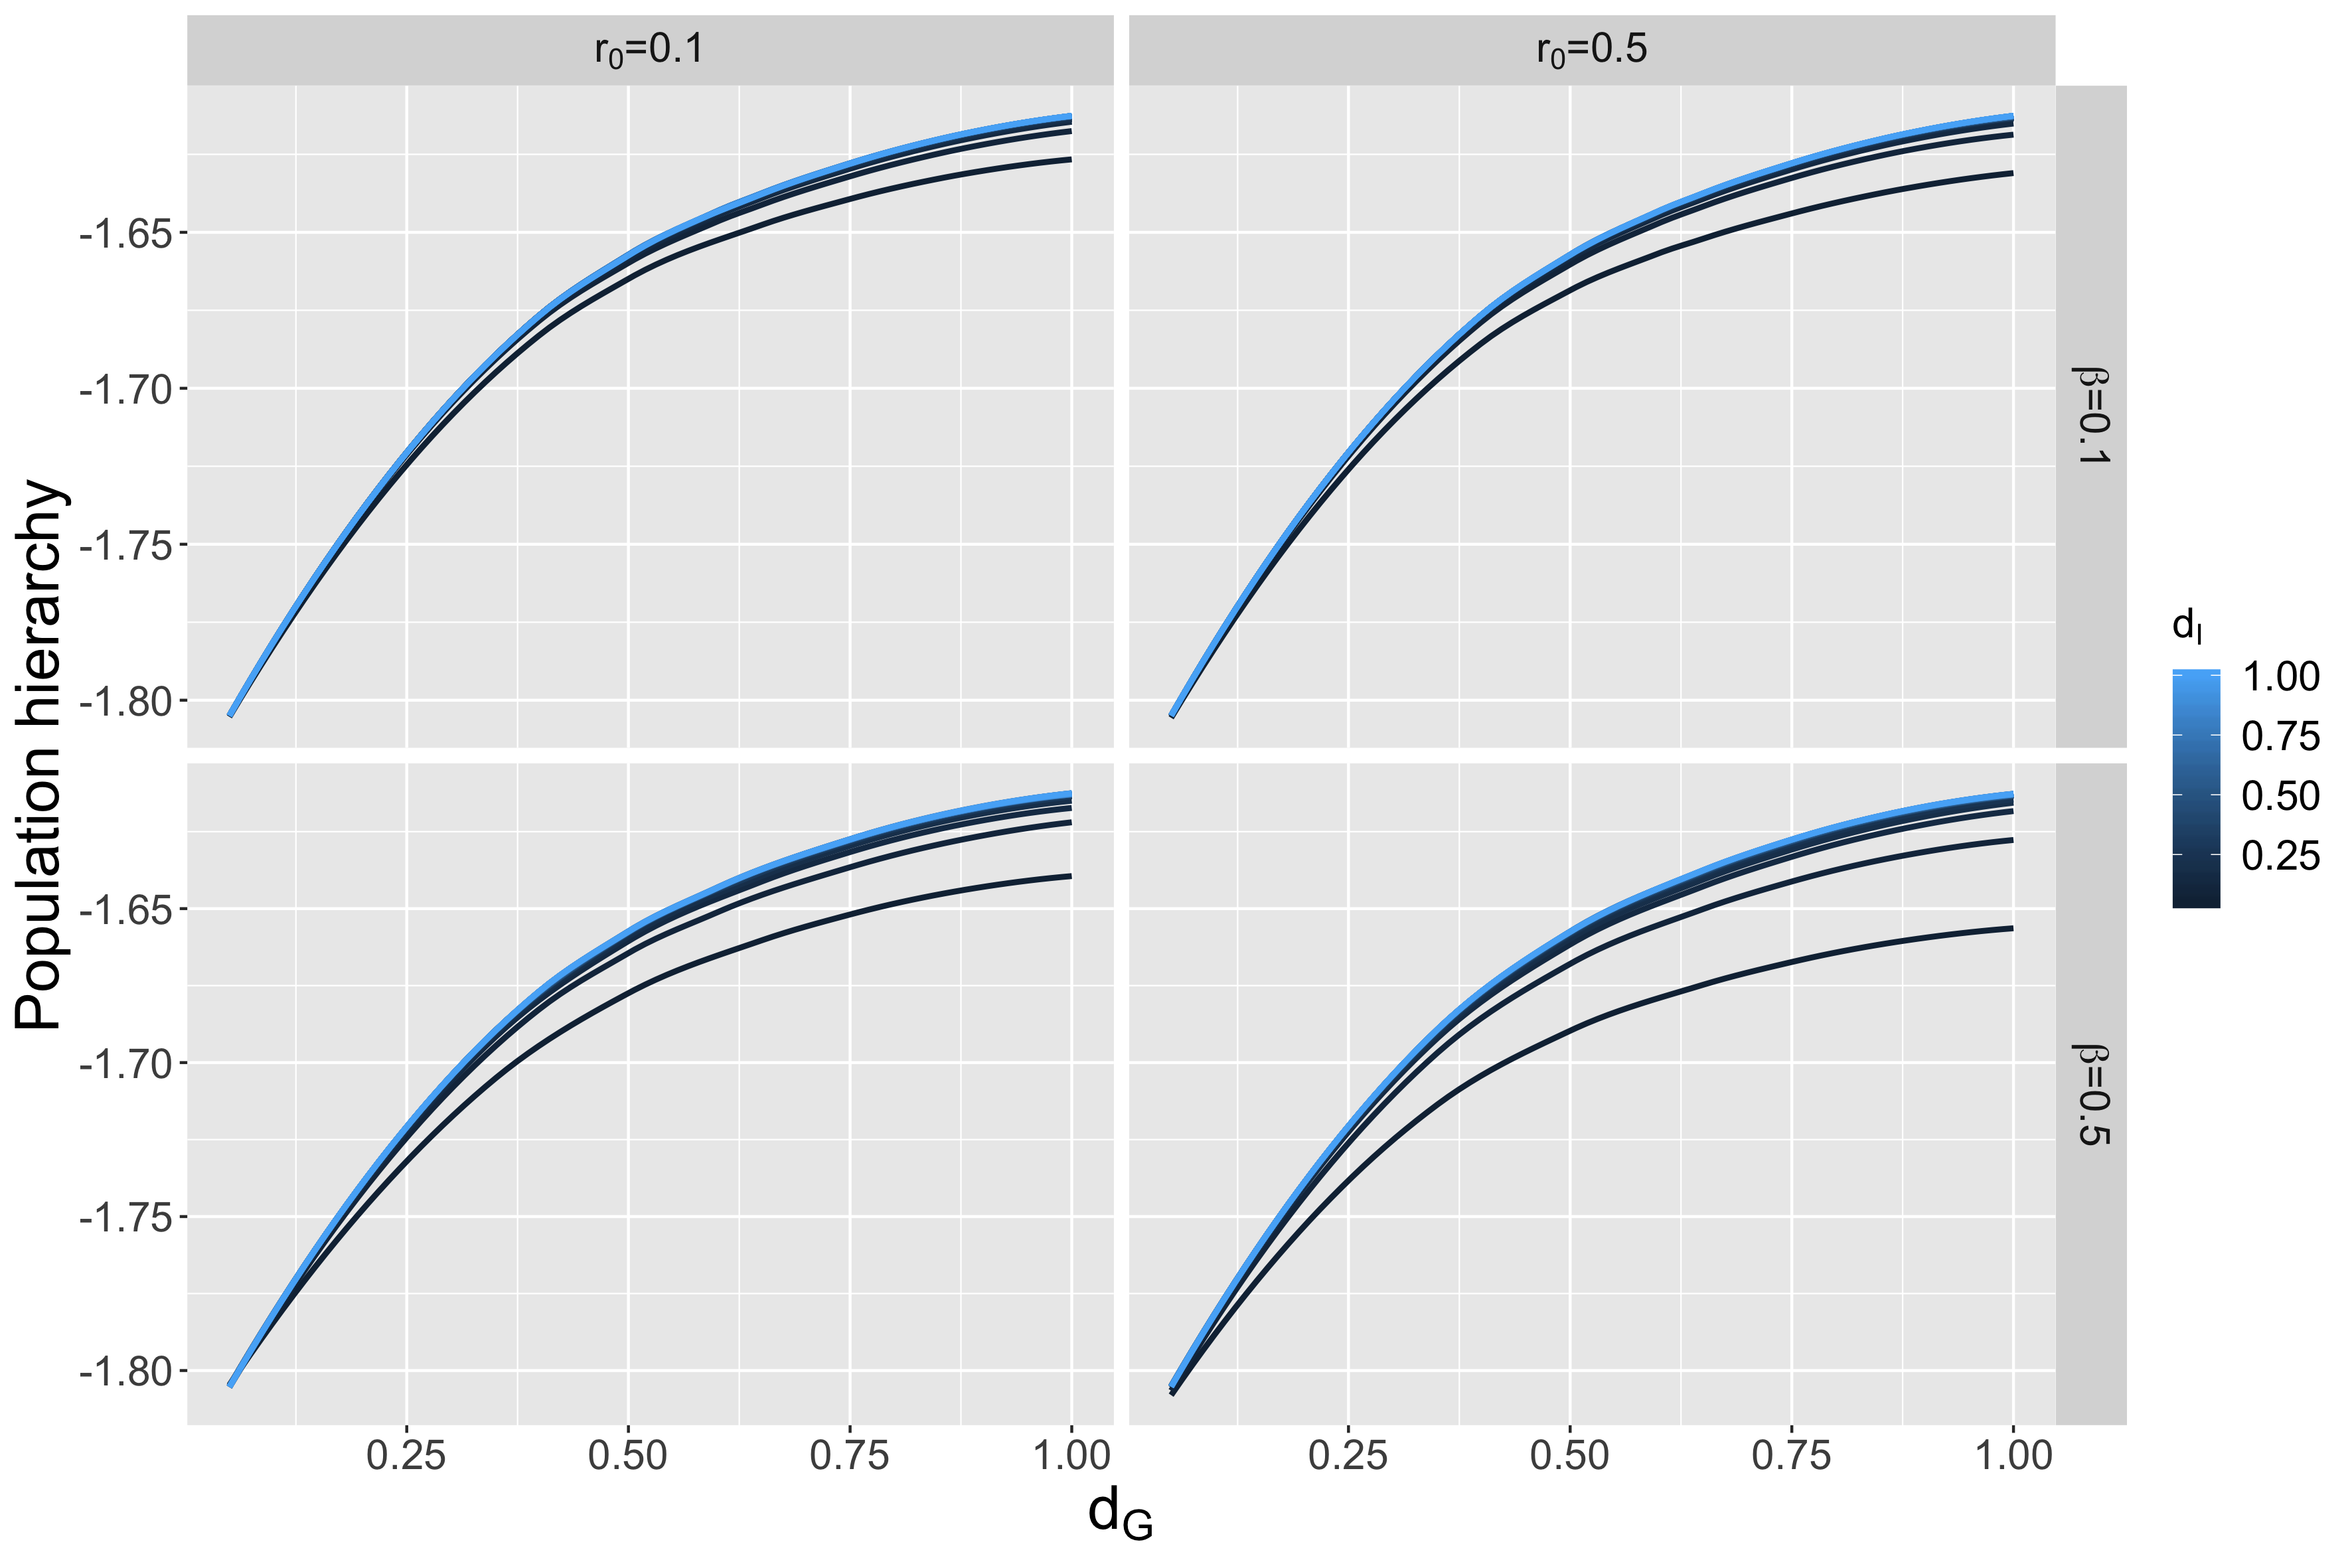
\includegraphics[width=0.47\linewidth]{../../../Communications/ALife2020/figures/finalHierarchy-gravityDecay_color-innovationDecay_facet-mutationRate-earlyAdoptersRate_newInnovationHierarchy1_utilityStd1_distriblog-normal.png}
\end{center}

\smallskip

\footnotesize

\textit{Systems with more interactions and diffusion are less unequal and innovate more}

}

\sframe{Model exploration: utility}{

\begin{center}
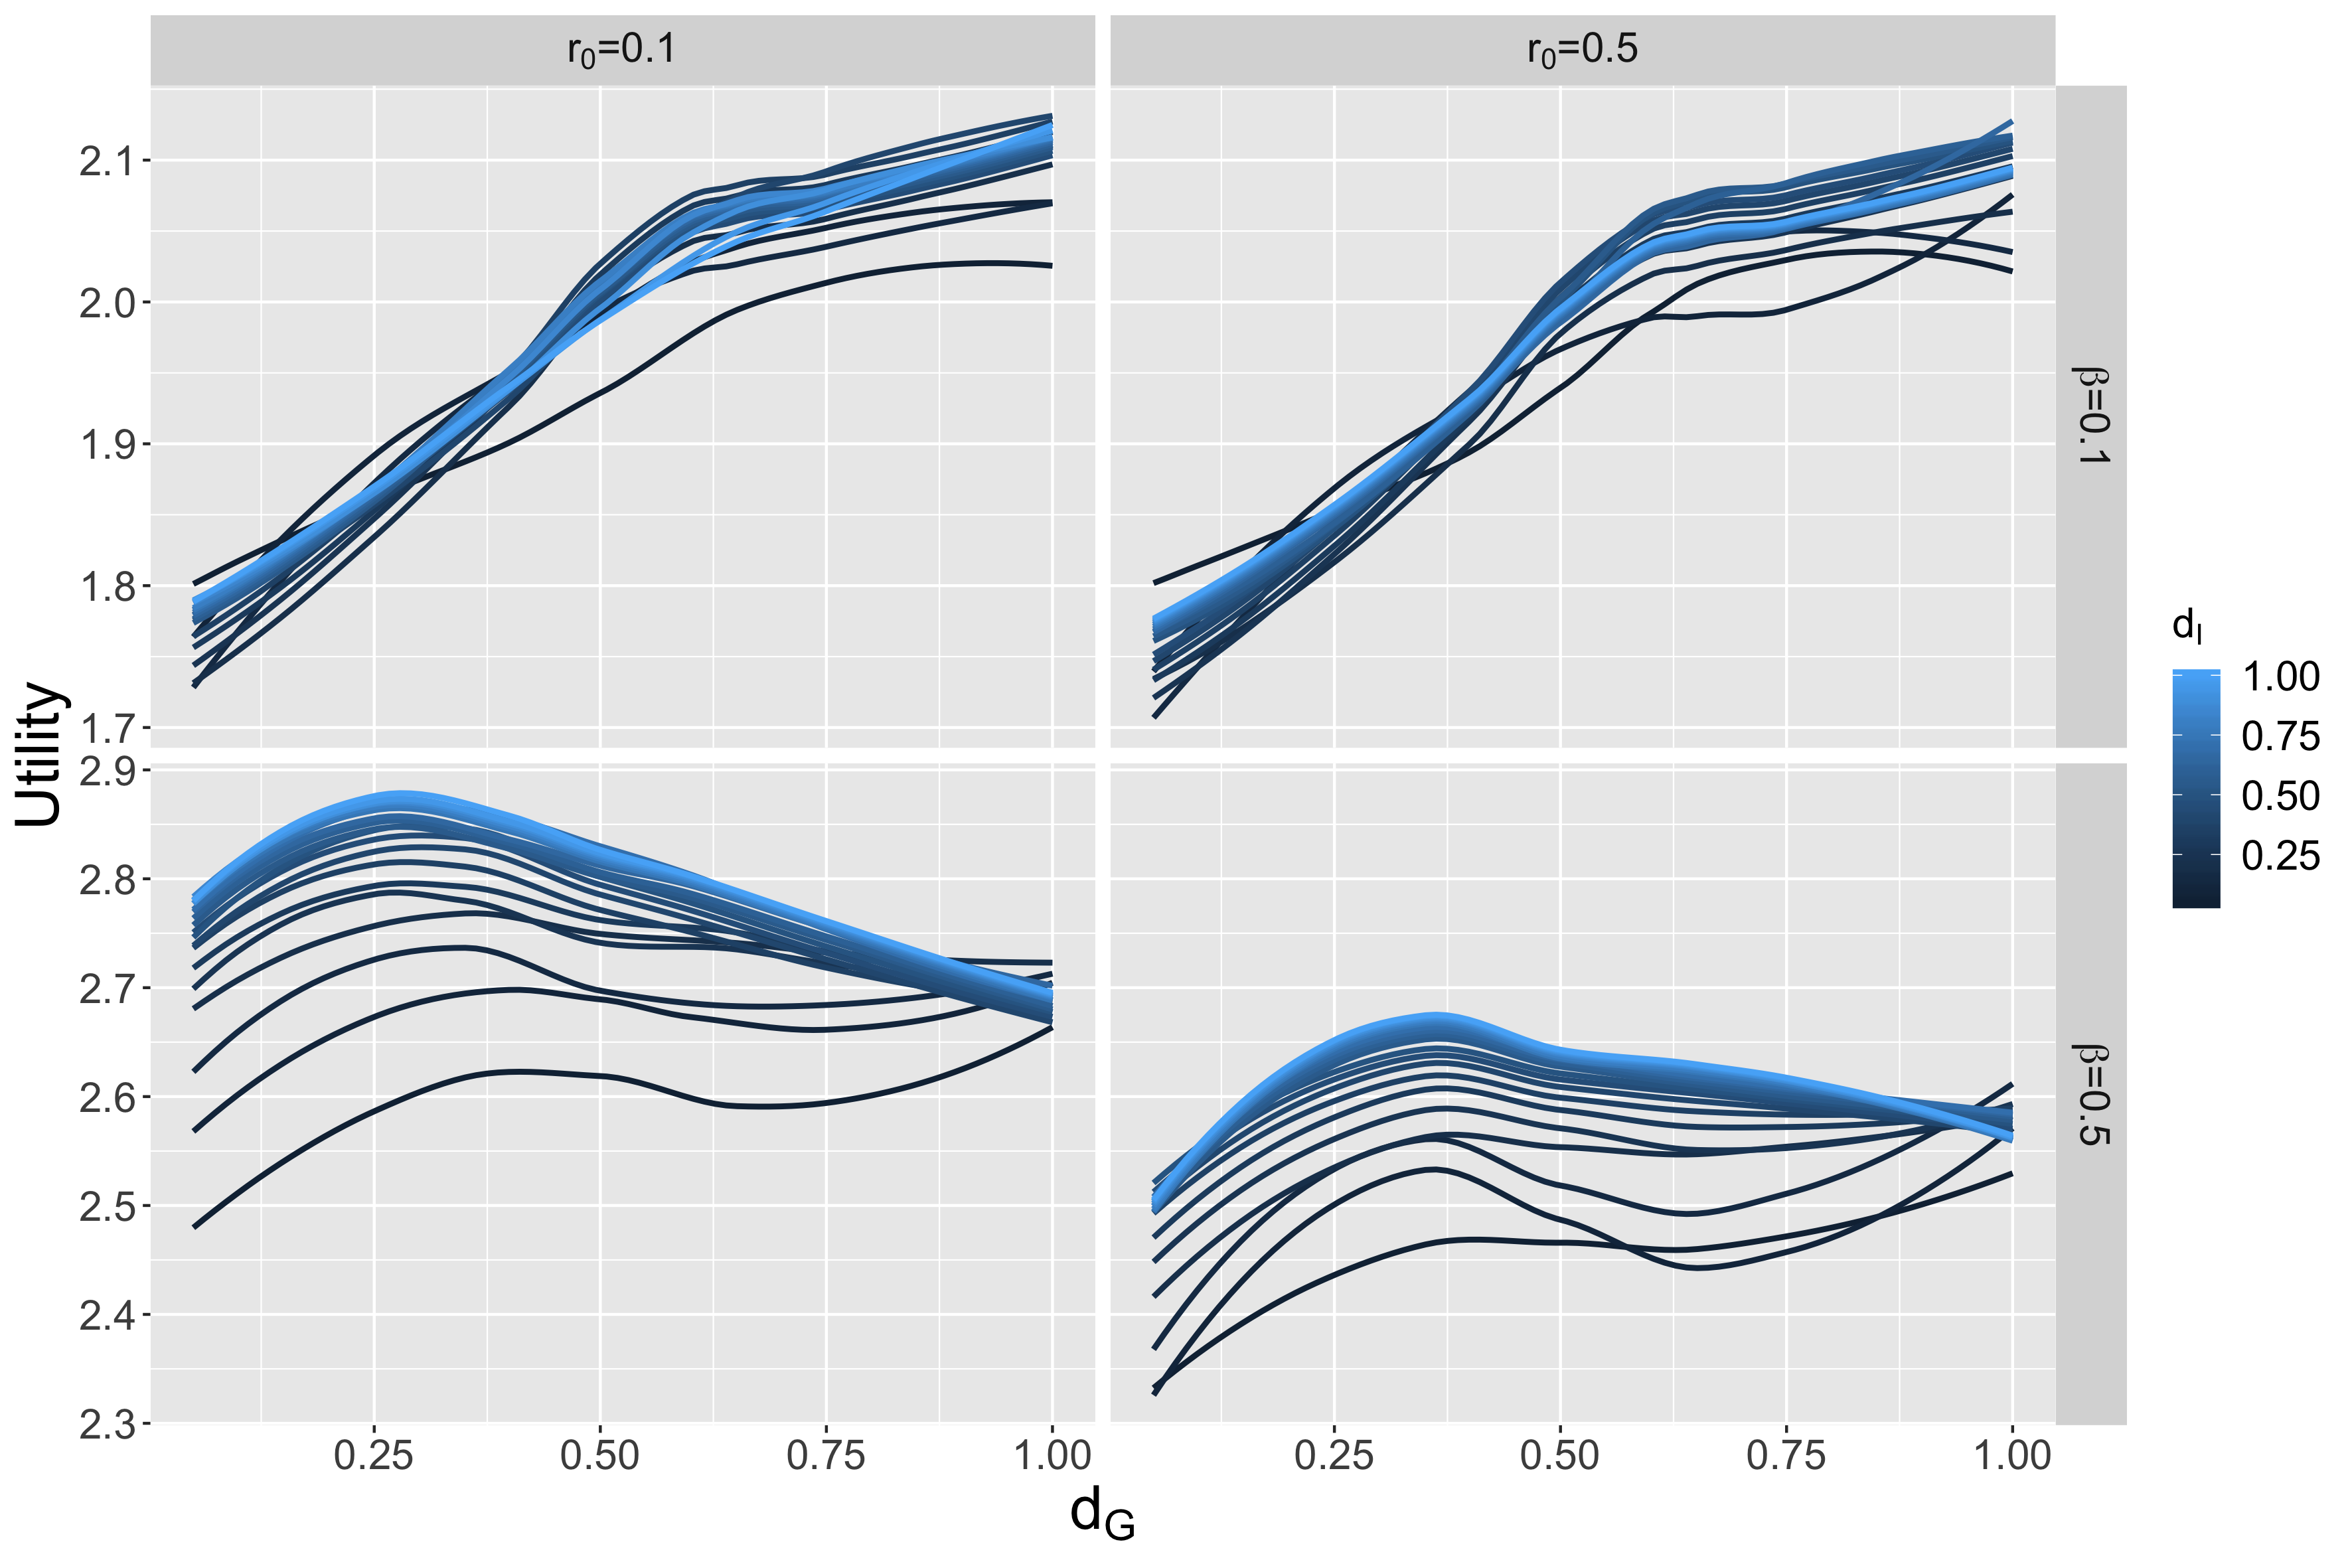
\includegraphics[width=0.8\linewidth]{../../../Communications/ALife2020/figures/averageUtility-gravityDecay_color-innovationDecay_facet-mutationRate-earlyAdoptersRate_newInnovationHierarchy1_utilityStd1_distriblog-normal.png}
\end{center}

\footnotesize

\textit{Piecewise behavior for low innovation rates; maximum as a function of $d_G$ for high innovation: emergence of regional innovation clusters?}

}




\sframe{Correlations}{

\begin{center}
	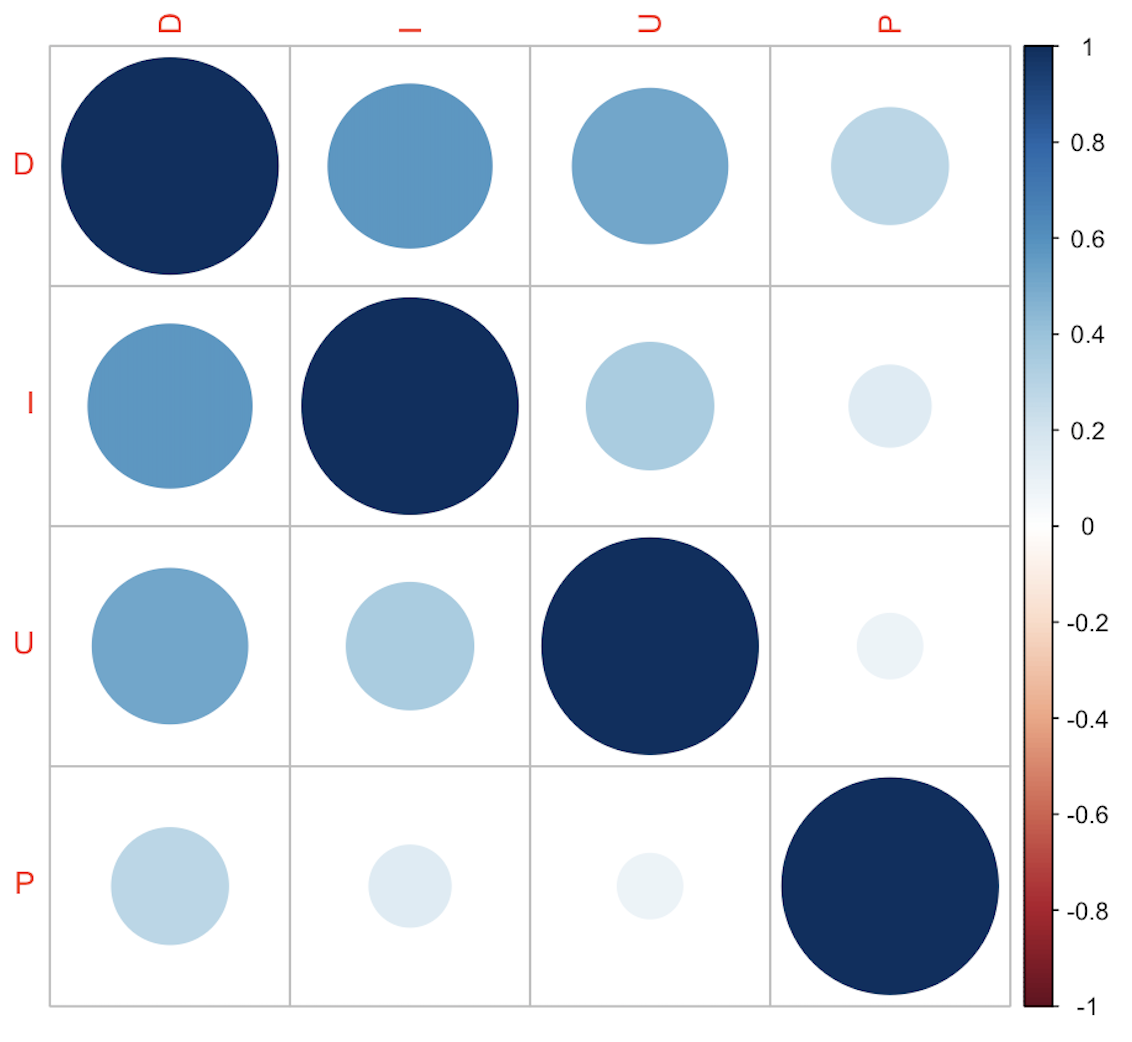
\includegraphics[width=0.6\linewidth]{../../../Communications/ALife2020/figures/corrmat_cropped.png}	
\end{center}

\footnotesize

\textit{Correlation matrix estimated over the whole exploration: innovation and population are not strongly correlated; 91\% of variance on first two components}

}


\sframe{Model optimization}{


\begin{center}
	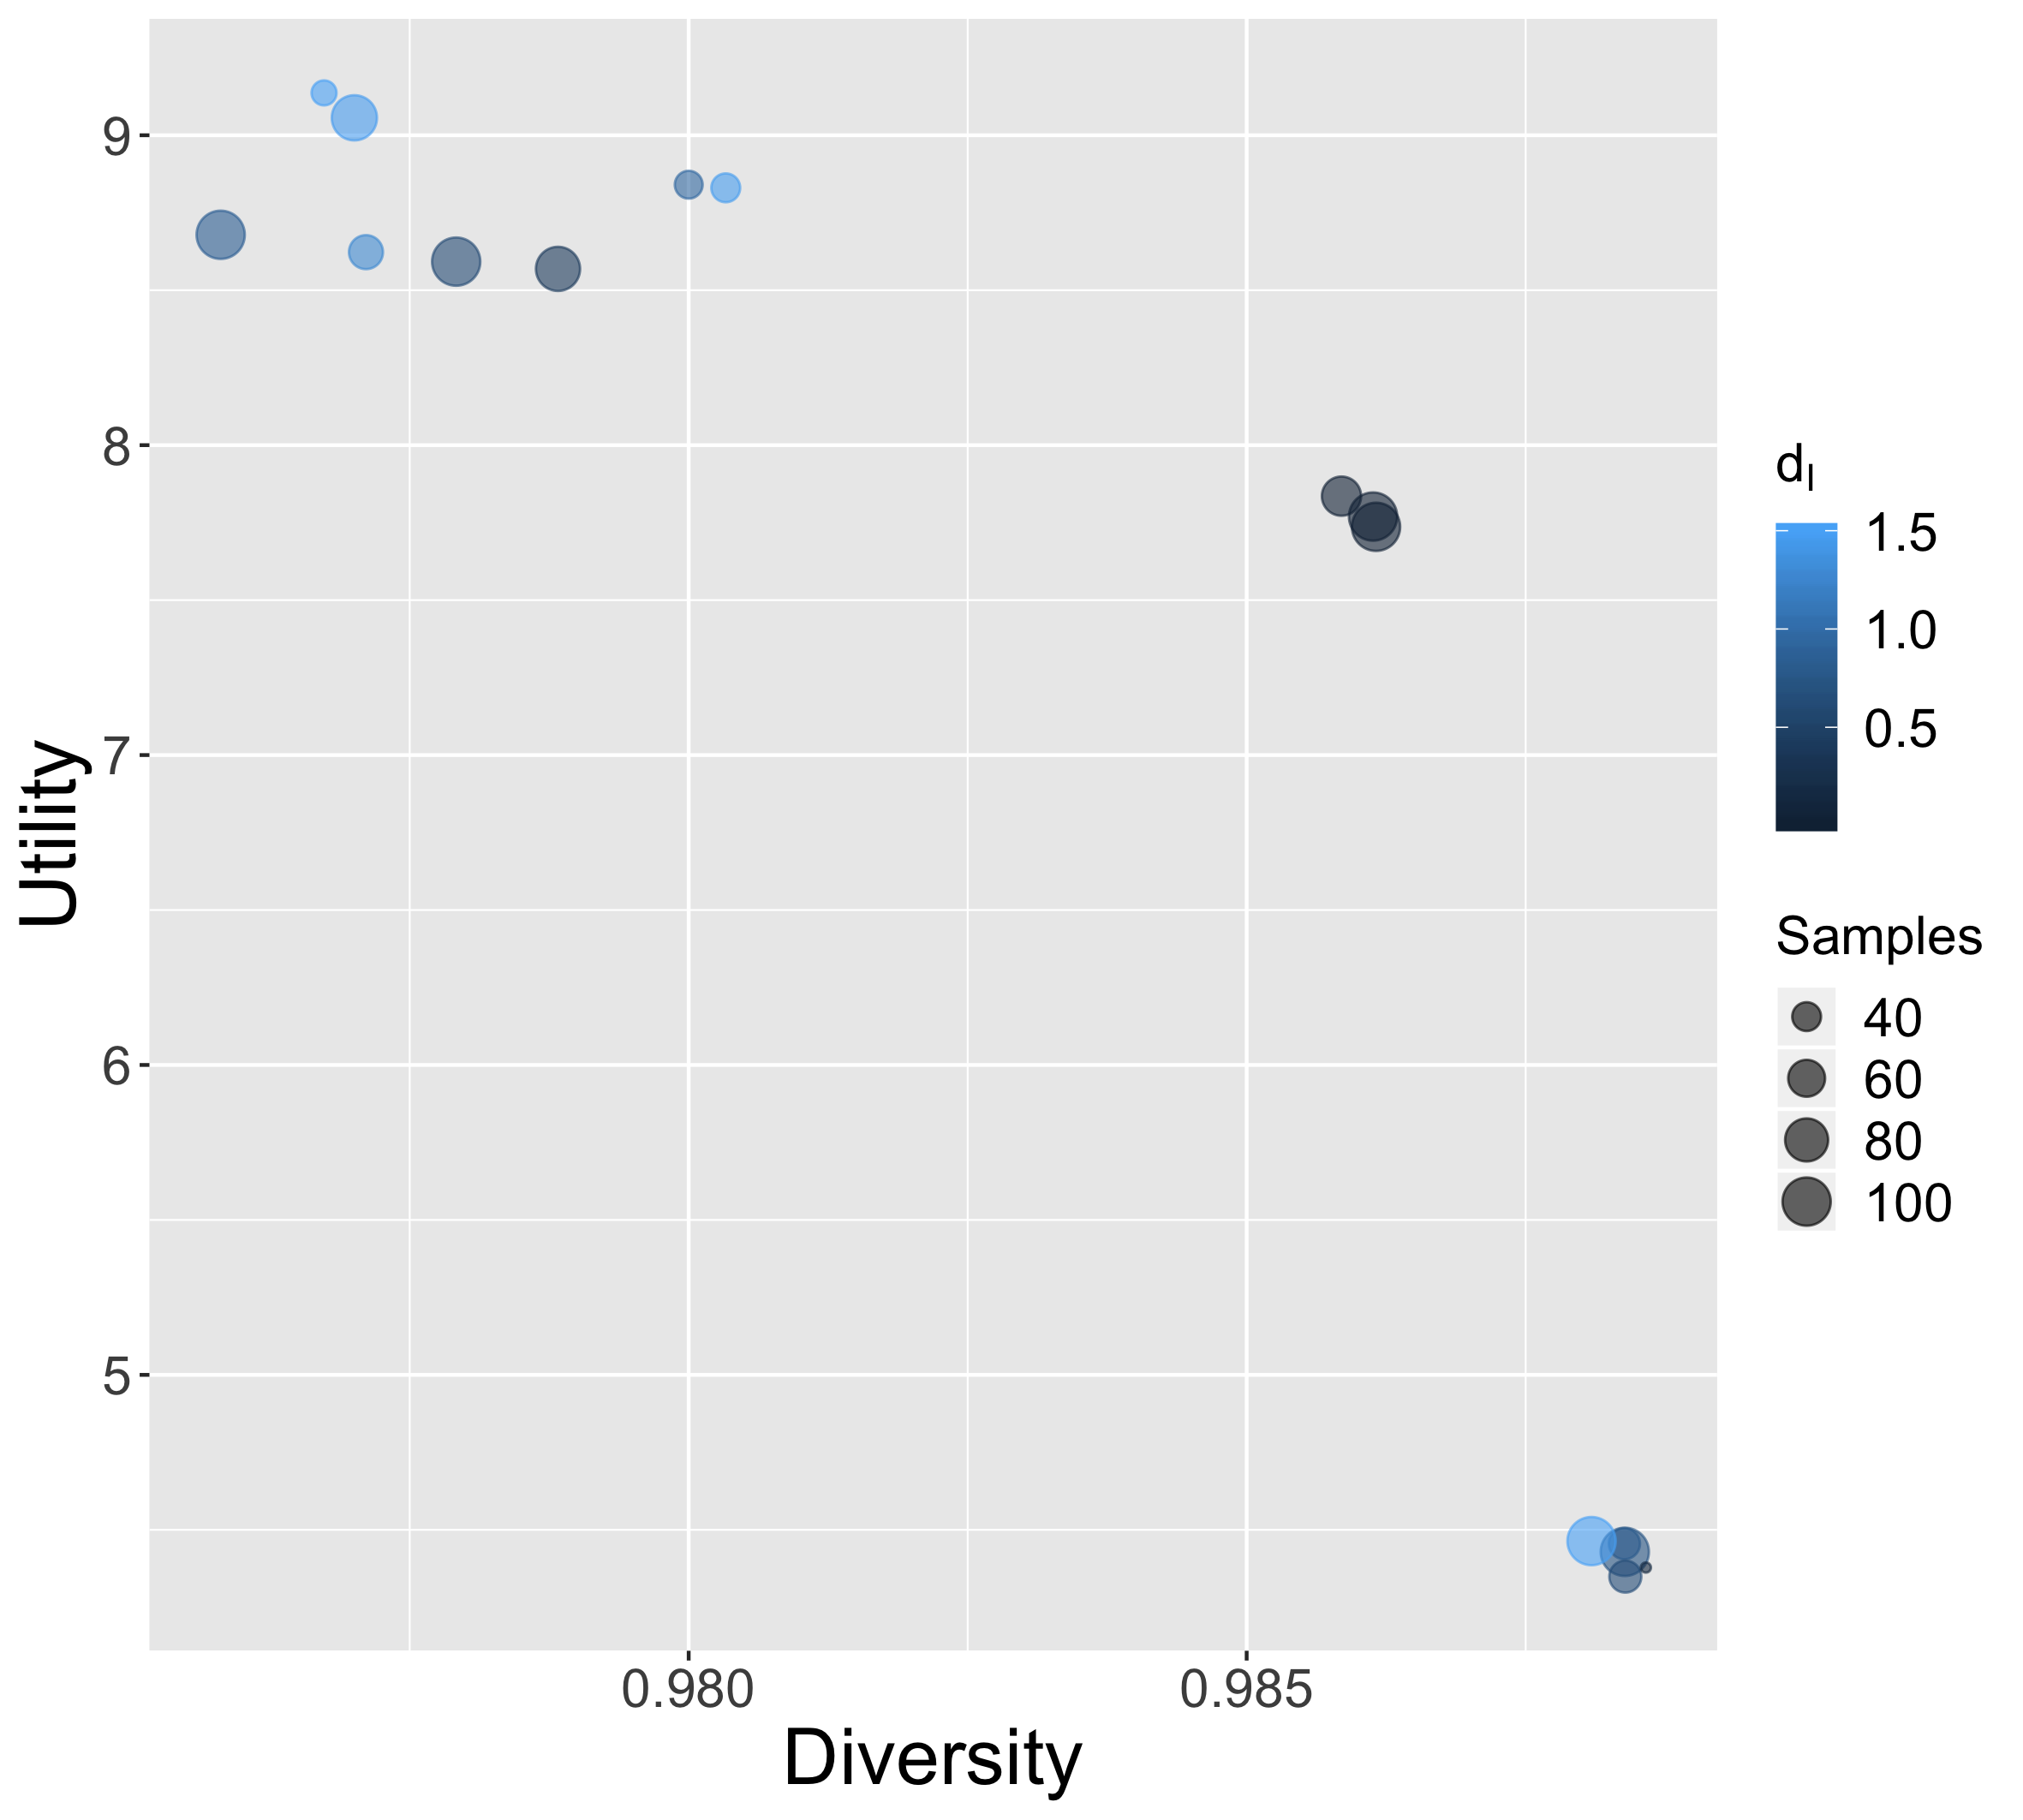
\includegraphics[width=0.6\linewidth]{../../../Communications/ALife2020/figures/paretoDiversity-Utility_colorinnovationDecay.png}
\end{center}

\footnotesize

\textit{NSGA2 algorithm to simultaneously optimize utility and diversity: emergence of three compromize regimes; intermediate regime with low level of innovation diffusion}




}



\sframe{Discussion}{

\textbf{Empirical and theoretical implications}

\smallskip

$\rightarrow$ Global integration of cities is not necessarily optimal in terms of overall utility

\smallskip

$\rightarrow$ Urban evolution simulation model including explicit evolution processes and an urban genome

\medskip

\textbf{Future work and extensions}

\smallskip

$\rightarrow$ Multi-dimensional urban genome to capture multi-dimensionality of urban dynamics \cite{hidalgo2007product}

\smallskip

$\rightarrow$ Application to real systems of cities \cite{2020arXiv200510007R}: patent data as possible proxy for innovation dynamics \cite{bergeaud2017classifying}

\smallskip

$\rightarrow$ Processes at other scales, towards multi-scale models \cite{raimbault:halshs-02351722}


%  A simple model of urban evolution capturing complex dynamics at the macroscopic scale through the diffusion of innovations

%$\rightarrow$ An ALife approach to the simulation of urban systems: ``Cities as they could be''

}





\section{Co-evolution in urban systems}


% The last part of the presentation focuses on the concept of co-evolution in urban systems, proposing a specific definition, a method to characterise it based on circular causations, and an application to the co-evolution between transportation networks and territories. For this particular case, we summarise results from co-evolution models at the mesoscopic scale (co-evolution between urban form and road networks) and at the macroscopic scale (co-evolution between cities and urban networks).



\sframe{Interactions between networks and territories}{

\justify

\begin{center}
\includegraphics[width=0.45\linewidth]{../../../../../CityNetwork/Docs/Communications/2019/TQGDebates2019/figures/accessp_withbridge_prd_EN.png}
\hspace{0.1cm}
\includegraphics[width=0.52\linewidth]{../../../../../CityNetwork/Docs/Communications/2019/TQGDebates2019/figures/avgaccess_facet.png}

\end{center}

\medskip

%\vspace{-0.5cm}

%\begin{justify}
\textit{Accessibility as part of complex processes of co-evolution between transportation networks and territories.}

%\end{justify}

\nocite{raimbault2018evolving}

\medskip

\tiny

Raimbault, J. (2019). Evolving accessibility landscapes: mutations of transportation networks in China. In Aveline-Dubach, N., ed. \textit{Pathways of sustainable urban development across China - the cases of Hangzhou, Datong and Zhuhai}, pp 89-108. Imago. ISBN:978-88-94384-71-0

}





\sframe{Definition of co-evolution \cite{raimbault2019modeling}}{

\footnotesize
 
  \textbf{Objects: } 
  
  \begin{itemize}
  	\item Cities and territories seen from the \textit{Evolutionary Urban Theory} viewpoint
  	\item Transportation networks as realisation of ``transactional projects'', following the \textit{Territorial Theory of Networks} \cite{dupuy1987vers}
  \end{itemize}
 
 \bigskip

\uncover<2->{

\textbf{Processes: }

\textit{A three-level definition for co-evolution: } 
\begin{enumerate}
	\item \textcolor{blue}{at the agent level}
	\item \textcolor{green}{at the agent population level (niches)}
	\item \textcolor{red}{at the global system level}
\end{enumerate}  

}

\bigskip

\uncover<3->{

\textbf{Corresponding approaches: }

\begin{enumerate}
	\item \textcolor{blue}{Empirical studies (microscopic level)}
	\item \textcolor{green}{Urban morphogenesis modeling (niche level)}
	\item \textcolor{red}{Urban evolutionary theory models (macroscopic level)}
\end{enumerate}

\smallskip

\tiny
Raimbault, J. (2019). Modeling interactions between transportation networks and territories: a co-evolution approach. arXiv preprint arXiv:1902.04802.

}
 
 
}



\sframe{Measuring co-evolution}{

\begin{center}
\includegraphics[width=\linewidth]{../../../../../CityNetwork/Docs/Seminars/20180109_LAET/figures/causality_regimes}
\end{center}

\medskip

\footnotesize

Raimbault, J. (2017). Identification de causalit{\'e}s dans des donn{\'e}es spatio-temporelles. SAGEO 2017 Proceedings. \textit{Translated as arXiv:1709.08684}
\nocite{raimbault2017identification}


}


\sframe{Illustration of the method}{

\centering

\includegraphics[height=0.9\textheight]{../../../../../CityNetwork/Docs/Seminars/20180109_LAET/figures/causality_twovars.pdf}

}



\sframe{Method validation}{

\includegraphics[width=\linewidth]{../../../../../CityNetwork/Docs/Seminars/20180109_LAET/figures/4-2-2-fig-causalityregimes-arma.jpg}

\medskip

\textit{Synthetic data: auto-regressive process with lag 2, cross terms parametrized by random $(a_1,a_2) \in [-0.1,0.1]$.}

}

\sframe{Application on model of \cite{raimbault2014hybrid}}{

\includegraphics[width=\textwidth]{../../../../../CityNetwork/Docs/Seminars/20180109_LAET/figures/regimes_1.png}

}


\sframe{Application on \textit{Grand Paris Express}}{

\begin{center}
\includegraphics[width=0.55\textwidth]{../../../../../CityNetwork/Docs/Seminars/20180109_LAET/figures/reseaux}
\includegraphics[width=0.45\textwidth]{../../../../../CityNetwork/Docs/Seminars/20180109_LAET/figures/1-2-1-fig-casestudies-empiricalres}
\end{center}

\smallskip

\textit{Anticipated effects on the new infrastructure on real estate prices}

}




\sframe{Modeling contributions}{
	
	\textbf{Macroscopic scale:}
	\begin{itemize}
		\item Interaction models between cities including transportation networks		
		$\rightarrow$ \textit{Evidence of network effects; exploration of interaction regimes}
	\end{itemize}

	\bigskip
	
	\uncover<2->{
	\textbf{Mesoscopic scale:}
	\begin{itemize}
		\item Morphogenesis model coupling urban form and network
		
		 $\rightarrow$ \textit{Complementarity of multiple processes; calibration at the first and second order}
		\item Exploration of an extended LUTI model including transportation governance
	\end{itemize}
}
	
}




\sframe{Form and function in territories}{

\textit{Which ontology to include more complex functional properties in mesoscopic morphogenesis models?}

\medskip

$\rightarrow$ Territorial systems as the strong coupling between territories and (potential and realized) networks \cite{dupuy1987vers}.

\medskip

$\rightarrow$ Networks convey functional notions of centralities and accessibility, among others; have furthermore proper topological properties.


}


\sframe{A Morphogenesis Model of co-evolution}{

\justify

\vspace{-1cm}

$\rightarrow$ Coupled grid population distribution and vector transportation network, following the core of \cite{raimbault2014hybrid}

\medskip

$\rightarrow$ Local morphological and functional variables determine a patch-value, driving new population attribution through preferential attachment; combined to population diffusion (reaction-diffusion processes studied before)


\medskip

$\rightarrow$ Network growth is also driven by morphological, functional and local network measures, following diverse heuristics corresponding to different processes (multi-modeling)

\medskip

\textit{Local variables and network properties induce feedback on both, thus a strong coupling capturing the \textbf{co-evolution}}

\bigskip

{
\tiny

Raimbault, J. (2019). An urban morphogenesis model capturing interactions between networks and territories. In The Mathematics of Urban Morphology (pp. 383-409). Birkhäuser, Cham.

\medskip

Raimbault, J. (2018). Multi-modeling the morphogenesis of transportation networks. In Artificial Life Conference Proceedings (pp. 382-383).

}


}



\sframe{Model: Specification}{

\includegraphics[width=\textwidth]{../../../../../CityNetwork/Docs/Communications/2019/TQGDebates2019/figures/coevol_mesocoevol}

}



\sframe{Network Generation}{

At fixed time steps :

\begin{enumerate}
	\item Add new nodes preferentially to new population and connect them
	\item \justify Variable heuristic for new links, among: nothing, random, gravity-based deterministic breakdown, gravity-based random breakdown (from \cite{schmitt2014modelisation}), cost-benefits (from \cite{louf2013emergence}), biological network generation (based on \cite{tero2010rules})
\end{enumerate}

\medskip

\centering

\frame{\includegraphics[height=0.31\textwidth]{../../../../../CityNetwork/Docs/Communications/2019/TQGDebates2019/figures/coevol_example-bio-process-1}}\hspace{0.2cm}
\frame{\includegraphics[height=0.31\textwidth]{../../../../../CityNetwork/Docs/Communications/2019/TQGDebates2019/figures/coevol_example-bio-process-1-tick80}}

\footnotesize

\textit{Intermediate stage for biological network generation}

}




\sframe{Generated Urban Shapes: Urban Form}{

\centering

\frame{\includegraphics[width=0.28\textwidth]{../../../../../CityNetwork/Docs/Communications/2019/TQGDebates2019/figures/coevol_example_synthsetup}}\hspace{0.1cm}
\frame{\includegraphics[width=0.28\textwidth]{../../../../../CityNetwork/Docs/Communications/2019/TQGDebates2019/figures/coevol_example_form-accessonly}}\hspace{0.1cm}
\frame{\includegraphics[width=0.28\textwidth]{../../../../../CityNetwork/Docs/Communications/2019/TQGDebates2019/figures/coevol_example_form-droadonly}}\\\vspace{0.1cm}
\frame{\includegraphics[width=0.28\textwidth]{../../../../../CityNetwork/Docs/Communications/2019/TQGDebates2019/figures/coevol_example_form-bwonly}}\hspace{0.1cm}
\frame{\includegraphics[width=0.28\textwidth]{../../../../../CityNetwork/Docs/Communications/2019/TQGDebates2019/figures/coevol_example_form-closenessonly}}\hspace{0.1cm}
\frame{\includegraphics[width=0.28\textwidth]{../../../../../CityNetwork/Docs/Communications/2019/TQGDebates2019/figures/coevol_example_form-poponly}}

\footnotesize\textit{In order: setup; accessibility driven; road distance driven; betweenness driven; closeness driven; population driven.}

}






\sframe{Generated Urban Shapes: Network}{


\centering

\frame{\includegraphics[width=0.28\textwidth]{../../../../../CityNetwork/Docs/Communications/2019/TQGDebates2019/figures/coevol_example_nw-connection}}\hspace{0.1cm}
\frame{\includegraphics[width=0.28\textwidth]{../../../../../CityNetwork/Docs/Communications/2019/TQGDebates2019/figures/coevol_example_nw-random}}\hspace{0.1cm}
\frame{\includegraphics[width=0.28\textwidth]{../../../../../CityNetwork/Docs/Communications/2019/TQGDebates2019/figures/coevol_example_nw-gravity}}\\\vspace{0.1cm}
\frame{\includegraphics[width=0.28\textwidth]{../../../../../CityNetwork/Docs/Communications/2019/TQGDebates2019/figures/coevol_example_nw-rndbrkdwn}}\hspace{0.1cm}
\frame{\includegraphics[width=0.28\textwidth]{../../../../../CityNetwork/Docs/Communications/2019/TQGDebates2019/figures/coevol_example_nw-cost}}\hspace{0.1cm}
\frame{\includegraphics[width=0.28\textwidth]{../../../../../CityNetwork/Docs/Communications/2019/TQGDebates2019/figures/coevol_example_nw-bio}}

\footnotesize\textit{In order: connection; random; deterministic breakdown; random breakdown; cost-driven; biological.}

}



\sframe{Results : Network Heuristics}{

\justify

\textit{Comparison of feasible space for network indicators with fixed density}

\bigskip

\includegraphics[width=0.52\textwidth,height=0.6\textheight]{../../../../../CityNetwork/Docs/Communications/2019/TQGDebates2019/figures/coevol_feasible_space_withreal_pca_bymorph}
\includegraphics[width=0.43\textwidth,height=0.6\textheight]{../../../../../CityNetwork/Docs/Communications/2019/TQGDebates2019/figures/coevol_distance_real_bymorph}

\footnotesize

\textit{(Left) Feasible spaces by morphological class and network heuristic; (Right) Distribution of distances to topologies of real networks}

}


\sframe{Results : Calibration}{

\justify

\vspace{-0.5cm}

Calibration (model explored with OpenMole~\cite{reuillon2013openmole}, $\sim 10^6$ model runs) at the first order on morphological and topological objectives, and on correlations matrices.

\bigskip

\begin{columns}
\column{0.4\textwidth}
\centering
\includegraphics[width=\textwidth]{../../../../../CityNetwork/Docs/Communications/2019/TQGDebates2019/figures/coevol_pca_allobjs}
\column{0.2\textwidth}
\includegraphics[width=\textwidth]{../../../../../CityNetwork/Docs/Communications/2019/TQGDebates2019/figures/coevol_pca_morpho_byheuristic}\\
\includegraphics[width=\textwidth]{../../../../../CityNetwork/Docs/Communications/2019/TQGDebates2019/figures/coevol_pca_network_byheuristic}
\column{0.4\textwidth}
\includegraphics[width=\textwidth]{../../../../../CityNetwork/Docs/Communications/2019/TQGDebates2019/figures/coevol_corrs-distrib_rhoasize4}

\end{columns}

\footnotesize\textit{(Left) Full indicator space; (Middle) Morphological and Topology, by network heuristic; (Right) Distance distribution for cumulated distance for indicators and correlations.}

}


\sframe{Results: Causality Regimes}{

\footnotesize
\textit{Unsupervised learning on lagged correlations between local variables unveils a diversity of causality regimes}

$\rightarrow$ Link between \emph{co-evolution regime} and morphogenetic properties of the urban system


\medskip

\begin{center}
\includegraphics[width=0.52\textwidth,height=0.55\textheight]{../../../../../CityNetwork/Docs/Communications/2019/TQGDebates2019/figures/coevol_centertrajs}
\includegraphics[width=0.4\textwidth,height=0.55\textheight]{../../../../../CityNetwork/Docs/Communications/2019/TQGDebates2019/figures/coevol_cluster-params}
\end{center}


\footnotesize

\textit{(Left) Lagged correlation profiles of cluster centers; (Right) Distribution of regimes across parameter space}

}




\sframe{Discussion}{

\justify

\vspace{-1cm}

\textbf{Implications}

$\rightarrow$ This rather simple model reproduces most of existing urban forms in Europe for both population distribution and road network: which intrinsic dimension to the urban system and its morphological aspect ?

$\rightarrow$ Ability to reproduce static correlations and a variety of dynamical lagged correlation regimes suggests that the model captures some of the processes of co-evolution


\bigskip

\textbf{Developments}


$\rightarrow$ Towards a dynamical calibration? Need for dynamical data

$\rightarrow$ Investigate the link between spatial non-stationarity and non-ergodicity through simulation by the model

$\rightarrow$ Compare network generation in a ``fair'' way (correcting for additional parameters, open question for models of simulation)


}



\sframe{Co-evolution of cities and networks}{

% simpopnet generator

\textit{Exploration of co-evolution regimes for the SimpopNet model}

\medskip

\begin{center}
\includegraphics[height=0.65\textheight]{../../../../../OpenMole/courses/spatialsens/figures/simpopnet_Fig1.png}
\end{center}

\tiny

Raimbault, J. (2020). Unveiling co-evolutionary patterns in systems of cities: a systematic exploration of the SimpopNet model. In Theories and Models of Urbanization (pp. 261-278). Springer, Cham.
\nocite{raimbault2020unveiling}

}




\sframe{Macroscopic co-evolution model}{

%\centering

\begin{center}
\includegraphics[width=0.95\textwidth]{../../../../../OpenMole/courses/spatialsens/figures/macrocoevol_en.png}
\end{center}


\tiny

Raimbault, J. (2020). Indirect evidence of network effects in a system of cities. Environment and Planning B: Urban Analytics and City Science, 47(1), 138-155.

\smallskip

Raimbault, J. (2020). Modeling the co-evolution of cities and networks. In Niel, Z., Rozenblat, C., eds. \textit{Handbook of Cities and Network}, Edwar Elgar Publishing, \textit{in press}. arXiv:1804.09430

\nocite{raimbault2020indirect}
\nocite{raimbault2018modeling}


}

\sframe{Model application}{

\begin{center}
\includegraphics[height=0.65\textheight]{../../../../../NetworksTerritories/CoevolutionNwTerritories/Docs/Papers/HierarchyCoevolution/chapter/figures/Fig1.png}\hspace{0.2cm}
\includegraphics[height=0.65\textheight]{../../../../../NetworksTerritories/CoevolutionNwTerritories/Docs/Papers/HierarchyCoevolution/chapter/figures/Fig4.png}
\end{center}

\smallskip

\tiny

Raimbault, J. (2020). Hierarchy and co-evolution processes in urban systems. arXiv preprint arXiv:2001.11989. Forthcoming in Fen-Chong, J. ed. Centralit{\'e}s et hi{\'e}rarchies des r{\'e}seaux et des territoires, ISTE Editions.
\nocite{raimbault2020hierarchy}

}



\sframe{Co-evolution regimes}{


\begin{center}

	\includegraphics[width=0.9\linewidth]{../../../../../CityNetwork/Docs/Seminars/20190617_PrixThese/figures/macro-regimes.png}
	\end{center}
	
	\medskip
	

\vspace{-0.4cm}

	\textit{Multiple co-evolution regimes unveiled for synthetic configurations}


}






\section{Discussion}


% We finally discuss perspectives towards more complex and multi-scalar models of urban evolution.


\sframe{Towards more complex models}{

\textit{The LUTECIA model includes transportation governance for network growth \cite{le2015modeling}}

\medskip

\centering
\includegraphics[width=\linewidth]{../../../../../CityNetwork/Docs/Seminars/20190617_PrixThese/figures/meso-lutecia.jpg}

}

\sframe{Towards more complex models}{

\textit{Including multinational transportation governance into the macroscopic co-evolution model}

\medskip

\begin{center}
\includegraphics[width=\linewidth]{../../../../../Governance/Docs/Communications/2020/CCS2020/communication/figures/ex_baseline_full.png}
\end{center}

\smallskip

\footnotesize

[Presentation yesterday at Conference on Complex Systems 2020]


}



\sframe{Towards multi-scale models}{

\justify

\textit{Crucial aspect of processes at multiple scales and feedback between these \cite{pumain2008socio}; need to be taken into account to build sustainable territorial policies \cite{rozenblat2018conclusion}}

\bigskip

$\rightarrow$ Empirical analysis of contradictory sustainability indicators on endogenous European mega-city regions \cite{raimbault2019multi}

\medskip

$\rightarrow$ A parsimonious multi-scalar urban growth model coupling spatial interactions at the macroscopic scale with reaction-diffusion models for urban form at the mesoscopic scale in \cite{raimbault:halshs-02351722}

\medskip

$\rightarrow$ Include physical transportation network in macroscopic co-evolution models \cite{raimbault2020hierarchy}


}



\sframe{Conclusion}{

\footnotesize

\textit{Urban evolution and co-evolution as a powerful paradigm to model, understand, sustainably manage urban systems}

\medskip

\footnotesize

\justify

\textbf{Open repositories for models} \texttt{https://github.com/JusteRaimbault/CityNetwork}

\texttt{https://github.com/JusteRaimbault/UrbanEvolution}


\medskip

\textbf{Acknowledgments}: \textit{European Grid Infrastructure}; UKCRIC DAFNI; Urban Dynamics Lab Grant EPSRC EP/M023583/1

\medskip

\textbf{References}

\tiny


Raimbault, J. (2017). Identification of causalities in spatio-temporal data. SAGEO 2017 Proceedings. arXiv:1709.08684
\nocite{raimbault2017identification}

\smallskip

Raimbault, J. (2018). Calibration of a density-based model of urban morphogenesis. PloS one, 13(9), e0203516.
\nocite{raimbault2018calibration}

\smallskip

Raimbault, J. (2018). Multi-modeling the morphogenesis of transportation networks. In Artificial Life Conference Proceedings (pp. 382-383).
\nocite{raimbault2018multi}

\smallskip

Raimbault, J. (2019). An urban morphogenesis model capturing interactions between networks and territories. In The Mathematics of Urban Morphology (pp. 383-409). Birkhäuser, Cham.

\nocite{raimbault2019urban}

\smallskip

Raimbault, J. (2019). Modeling interactions between transportation networks and territories: a co-evolution approach. arXiv preprint arXiv:1902.04802.
\nocite{raimbault2019modeling}

\smallskip

Raimbault, J. (2020). Unveiling co-evolutionary patterns in systems of cities: a systematic exploration of the SimpopNet model. In Theories and Models of Urbanization (pp. 261-278). Springer, Cham.
\nocite{raimbault2020unveiling}

\smallskip

Raimbault, J. (2020). Indirect evidence of network effects in a system of cities. Environment and Planning B: Urban Analytics and City Science, 47(1), 138-155.
\nocite{raimbault2020indirect}

\smallskip

Raimbault, J. (2020). Modeling the co-evolution of cities and networks. Handbook of cities and networks, Rozenblat C., Niel Z., eds. (in press) arXiv:1804.09430.
\nocite{raimbault2018modeling}

\smallskip

Raimbault, J. (2020). Hierarchy and co-evolution processes in urban systems. arXiv preprint arXiv:2001.11989. Forthcoming in Fen-Chong, J. ed. Centralit{\'e}s et hi{\'e}rarchies des r{\'e}seaux et des territoires, ISTE Editions.
\nocite{raimbault2020hierarchy}

}





%%%%%%%%%%%%%%%%%%%%%
\begin{frame}[allowframebreaks]
\frametitle{References}
\bibliographystyle{apalike}
\bibliography{biblio}
\end{frame}
%%%%%%%%%%%%%%%%%%%%%%%%%%%%










\end{document}

